\documentclass{article}
\usepackage{ctex}

\title{数字逻辑与计算机组成\\ {\small 实验 2: 组合逻辑电路设计}}
\author{王卫东\quad 221900332}
\date{\zhtoday}

\usepackage{hyperref}
\usepackage{algorithm}
\usepackage{algorithmicx}
\usepackage{algpseudocode}
\usepackage{float}  
\usepackage{lipsum}
\usepackage{color, xcolor}
\usepackage{listings}
\usepackage{dirtree}
\usepackage{ulem}
\usepackage{graphicx}
\usepackage{amsmath}
\usepackage{amssymb}
\usepackage{amsfonts}
\usepackage{xcolor}
\usepackage{tikz}
\usepackage{zhnumber} % change section number to chinese
\renewcommand\thesection{\zhnum{section}}
\renewcommand\thesubsection{\arabic{subsection}}
\usetikzlibrary{arrows,shapes,chains}

\begin{document}
    \maketitle

    \section{实验目的}

    \begin{enumerate}
        \item 掌握组合逻辑电路的设计方法和步骤,实现译码器、编码器等基本组合逻辑电路。
        \item 掌握串行加法器设计方法,理解减法和比较运算的实现方法。
        \item 掌握汉明码校验电路的设计方法。
    \end{enumerate}

    \section{实验环境}

    Logisim 2.16

    \section{实验内容}
    
    \subsection{译码器实验}

    \subsubsection{整体方案设计}
    \begin{figure}[H]
    \centering
    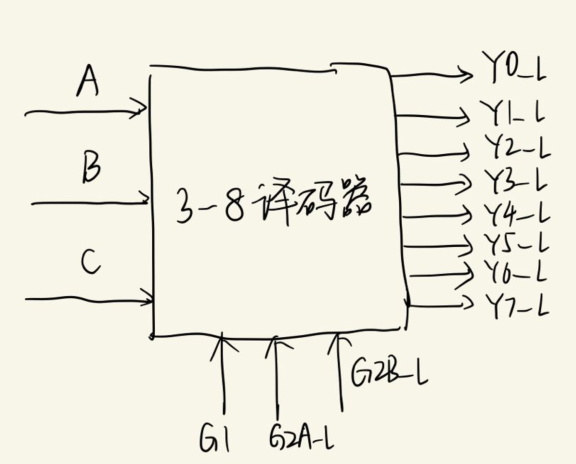
\includegraphics[width=0.8\textwidth]{1.1.png}
    \caption{3-8译码器整体方案设计}
    \end{figure}

    \subsubsection{顶层模块设计}
    实验电路较为简单,不需要顶层模块设计图。

    \subsubsection{引脚作用}
    \begin{table}[H]
    \centering
    \begin{tabular}{|c|c|}
        \hline
        A,B,C & 输入引脚 \\ \hline
        $Yi_L(0\le i\le 7)$   & 输出引脚 \\ \hline
        $G1\ G2A_L\ G2B_L$   & 使能端 \\ \hline
    \end{tabular}
    \caption{3-8译码器引脚作用}
    \end{table}

    \subsubsection{原理图和电路图}
    \begin{figure}[H]
    \centering
    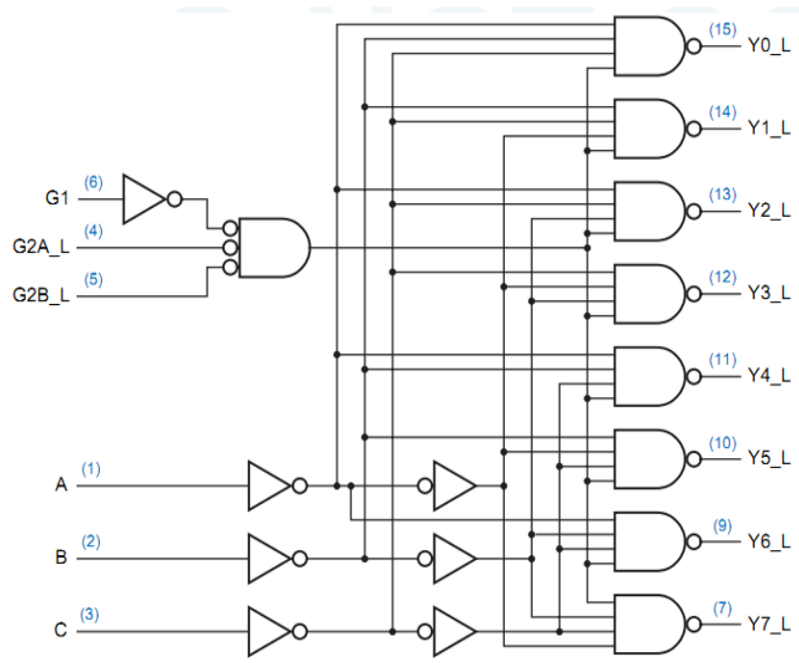
\includegraphics[width=0.8\textwidth]{1.4.1.png}
    \caption{3-8译码器原理图}
    \end{figure}

    \begin{figure}[H]
    \centering
    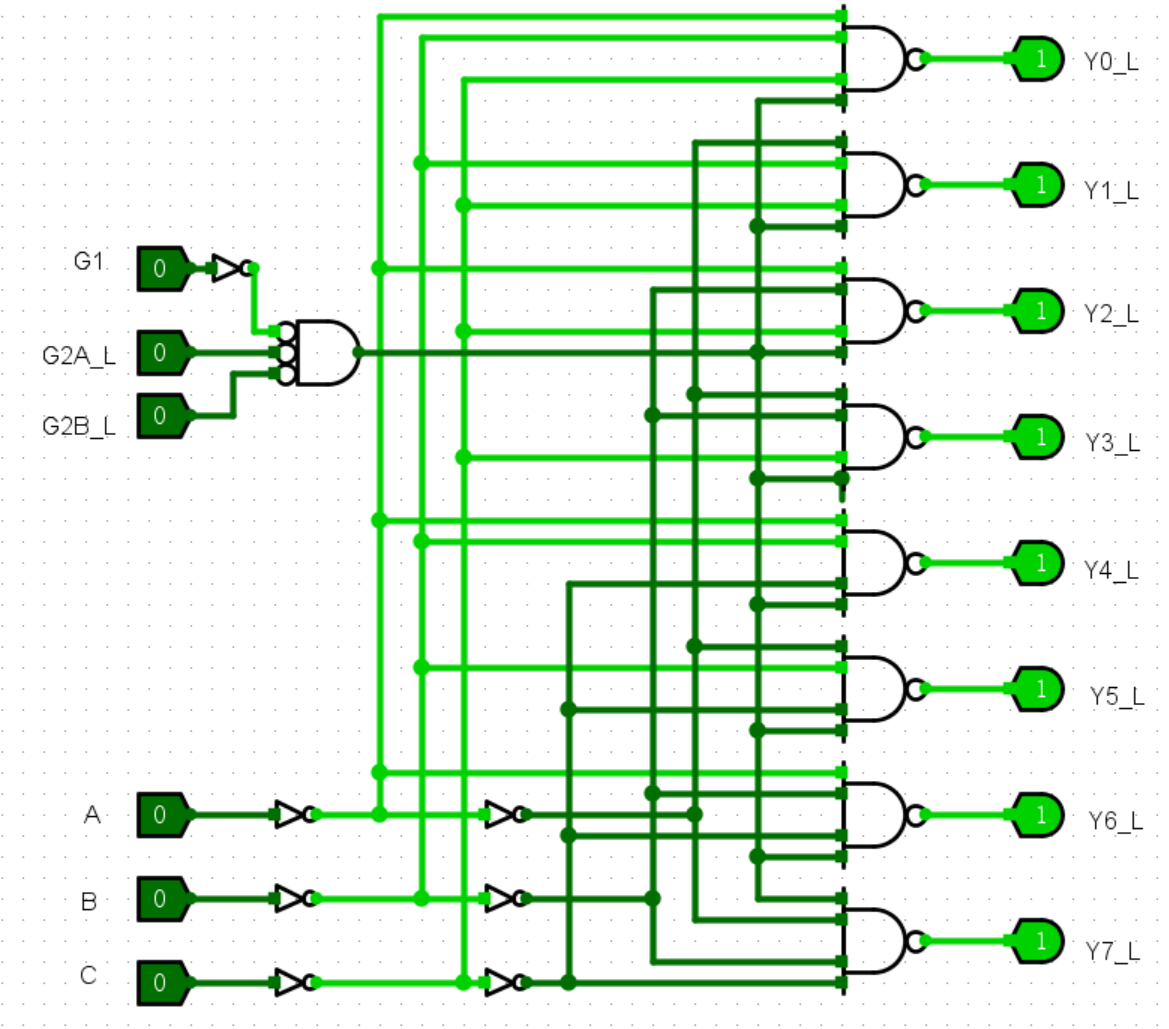
\includegraphics[width=0.8\textwidth]{1.4.2.png}
    \caption{3-8译码器电路图}
    \end{figure}

    \subsubsection{仿真测试图}
    \begin{figure}[H]
    \centering
    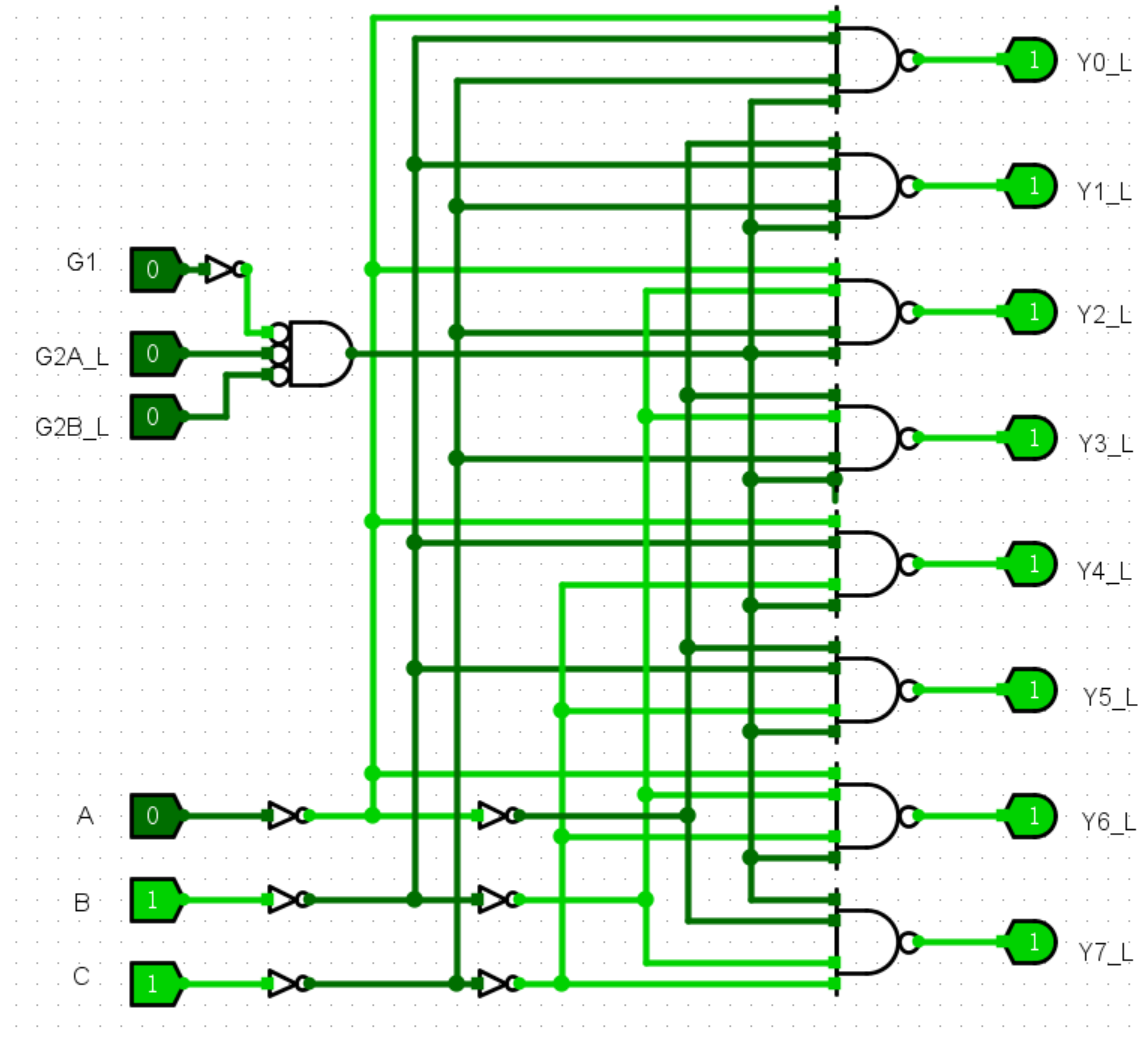
\includegraphics[width=0.4\textwidth]{1.5.1.png}
    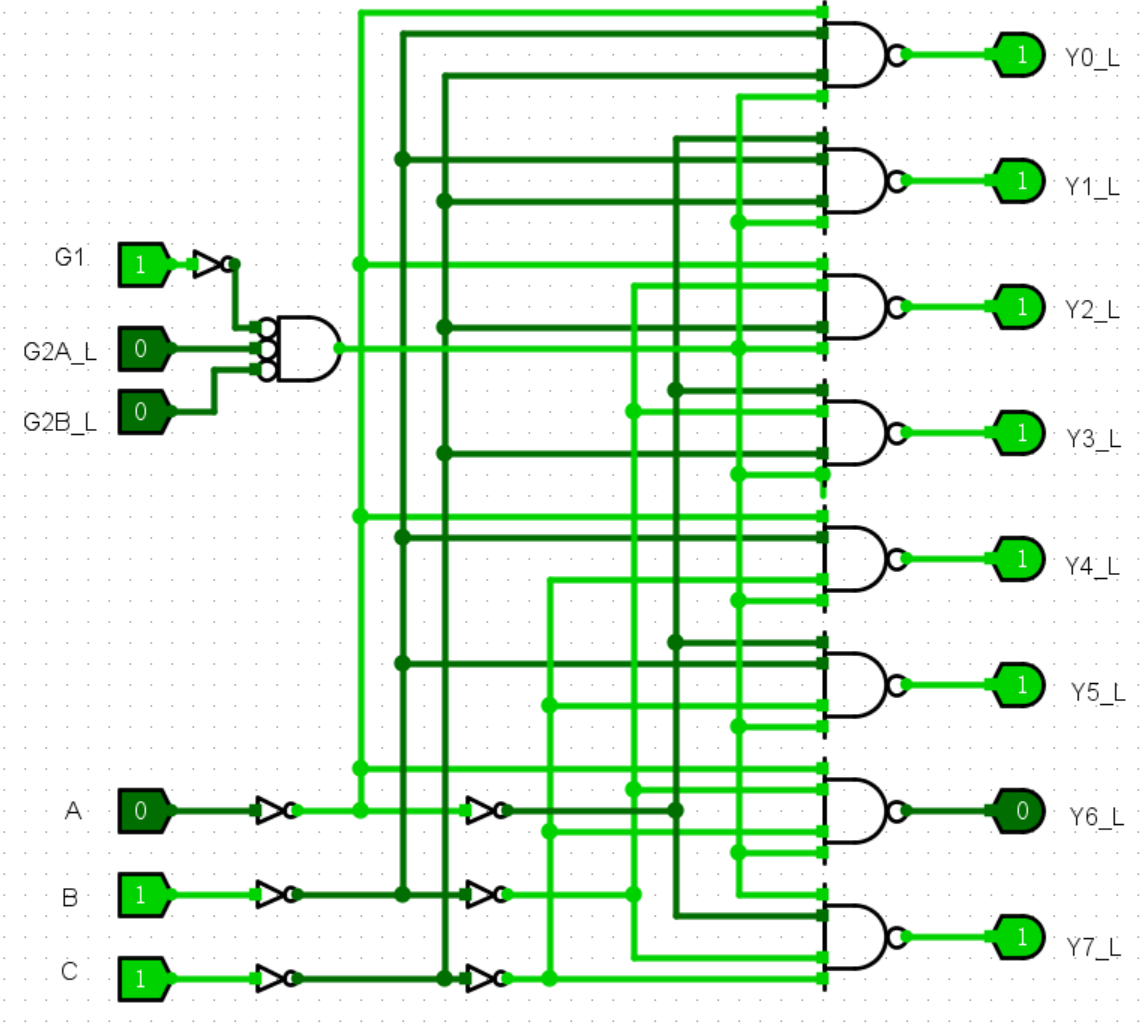
\includegraphics[width=0.4\textwidth]{1.5.2.png}
    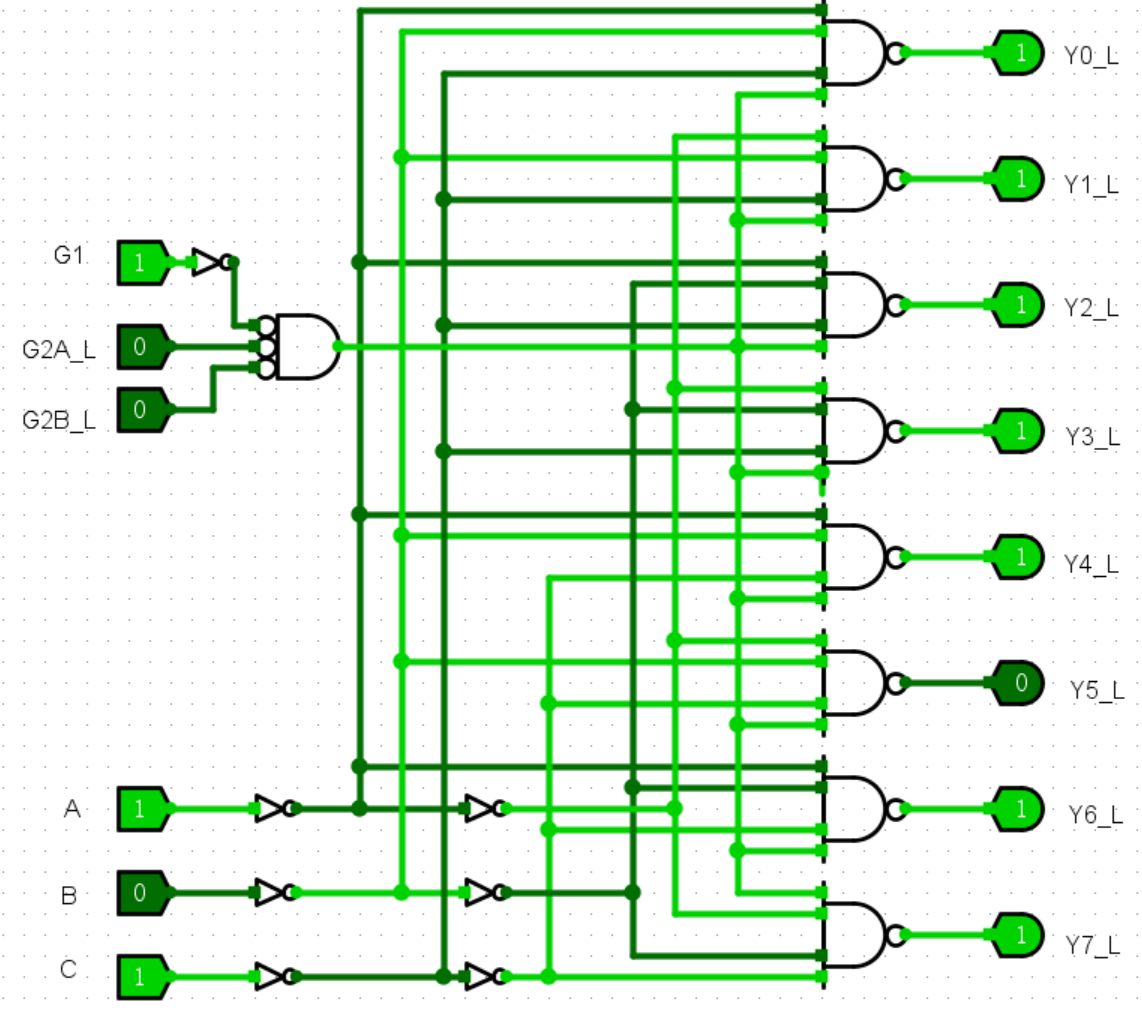
\includegraphics[width=0.4\textwidth]{1.5.3.png}
    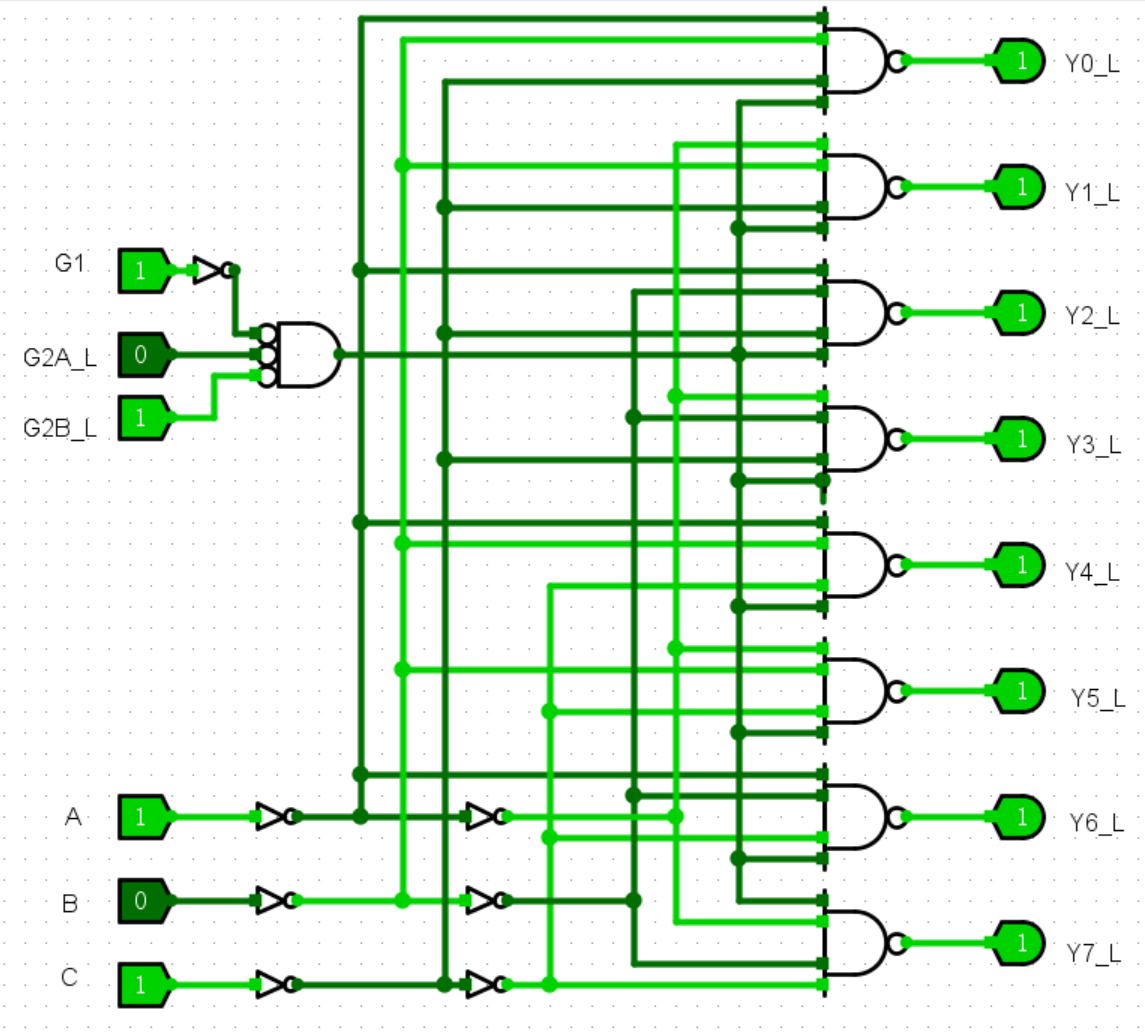
\includegraphics[width=0.4\textwidth]{1.5.4.png}
    \caption{3-8译码器仿真测试图}
    \end{figure}
    功能表如下。

    \begin{table}[H]
    \centering
    \begin{tabular}{|c|c|c|}
        \hline
        $使能端G1、G2A_L、G2B_L$ & $输入端ABC$ & 输出 \\ \hline
        0xx & xxx & 全置1 \\ \hline
        11x & xxx & 全置1 \\ \hline
        1x1 & xxx & 全置1 \\ \hline
        100 & 000 & $Y0_L$置0,其余置1 \\ \hline
        100 & 001 & $Y1_L$置0,其余置1 \\ \hline
        100 & 010 & $Y2_L$置0,其余置1 \\ \hline
        100 & 011 & $Y3_L$置0,其余置1 \\ \hline
        100 & 100 & $Y4_L$置0,其余置1 \\ \hline
        100 & 101 & $Y5_L$置0,其余置1 \\ \hline
        100 & 110 & $Y6_L$置0,其余置1 \\ \hline
        100 & 111 & $Y7_L$置0,其余置1 \\ \hline
    \end{tabular}
    \caption{3-8译码器功能表}
    \end{table}

    \subsubsection{错误现象及分析}
    在完成实验的过程中,没有遇到任何错误。
    
    \subsection{编码器实验}

    \subsubsection{整体方案设计}
    \begin{figure}[H]
    \centering
    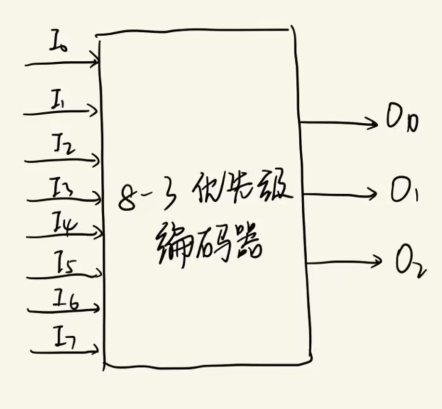
\includegraphics[width=0.8\textwidth]{2.1.png}
    \caption{8-3优先级编码器整体方案设计}
    \end{figure}
    \subsubsection{顶层模块设计}
    实验电路较为简单,不需要顶层模块设计图。

    \subsubsection{引脚作用}
    \begin{table}[H]
    \centering
    \begin{tabular}{|c|c|}
        \hline
        $I_{0}$ ~ $I_{7}$ & 输入引脚 \\ \hline
        $O_{0}$ $O_{1}$ $O_{2}$   & 输出引脚 \\ \hline
    \end{tabular}
    \caption{8-3优先级编码器引脚作用}
    \end{table}

    \subsubsection{原理图和电路图}
    \begin{figure}[H]
    \centering
    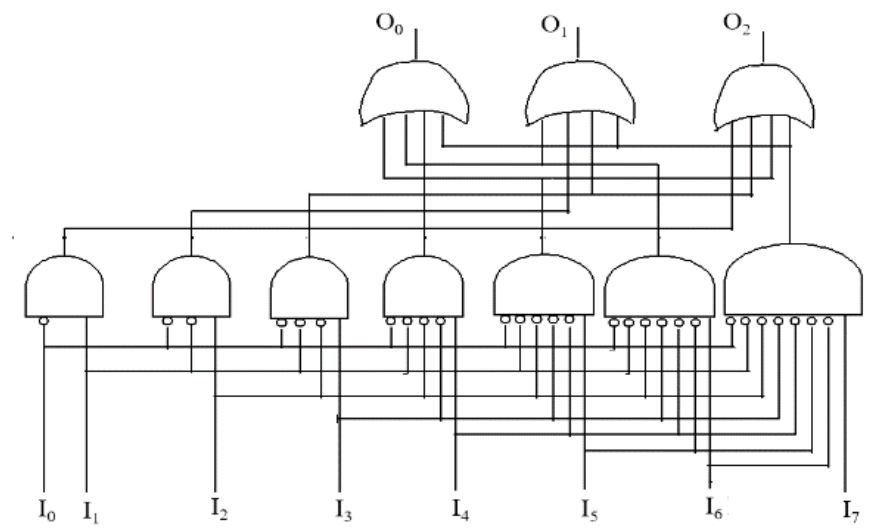
\includegraphics[width=0.8\textwidth]{2.4.1.png}
    \caption{8-3优先级编码器原理图}
    \end{figure}

    \begin{figure}[H]
    \centering
    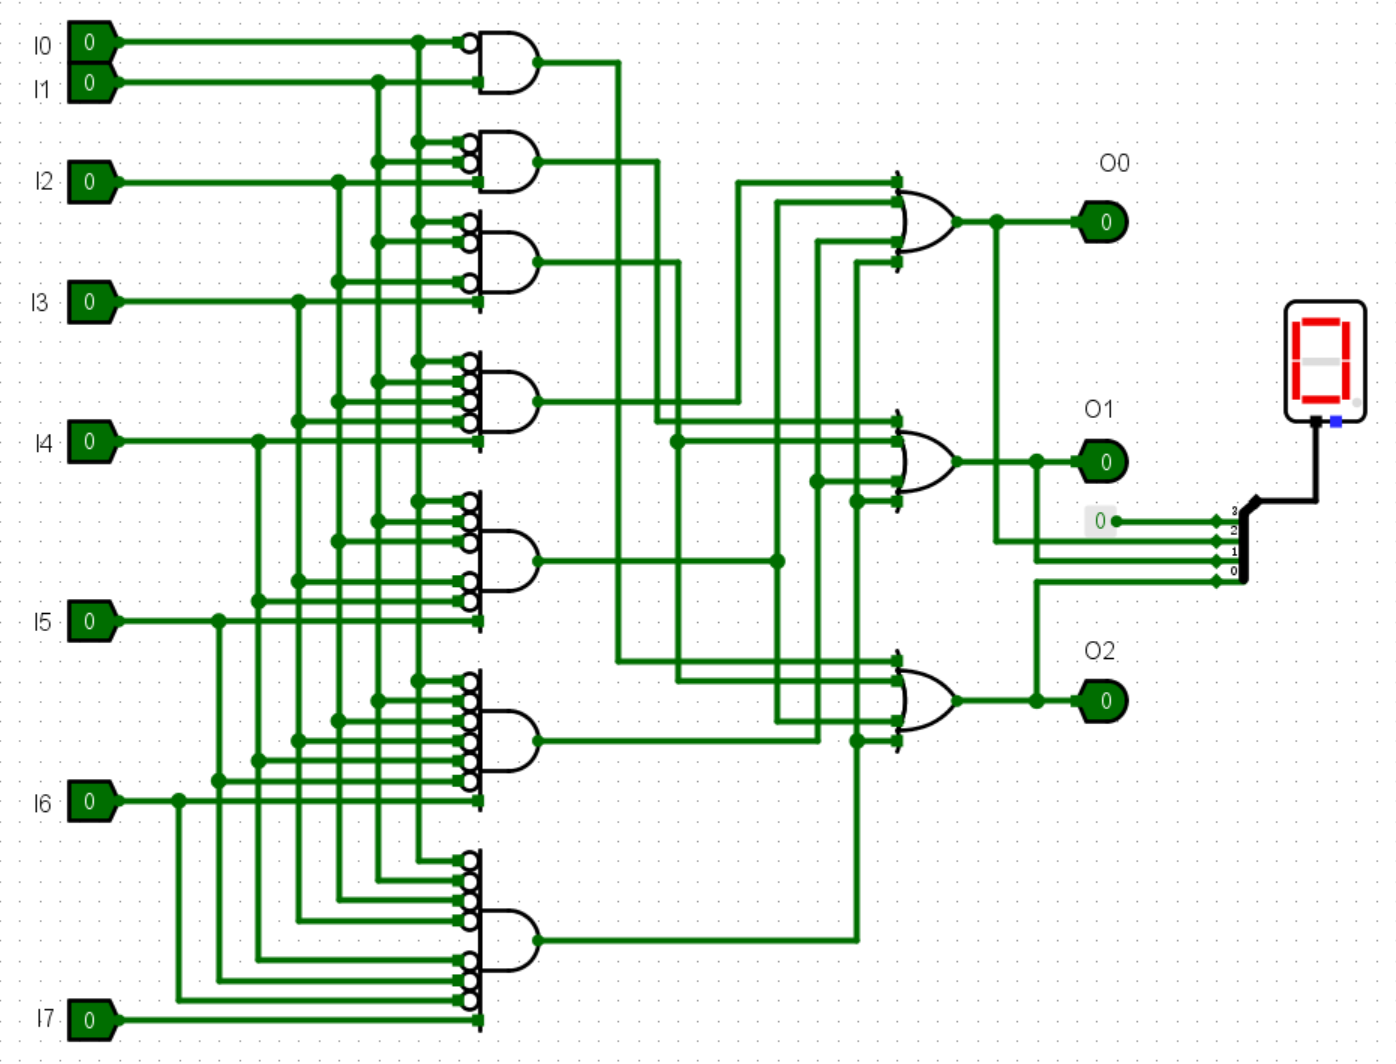
\includegraphics[width=0.8\textwidth]{2.4.2.png}
    \caption{8-3优先级编码器电路图}
    \end{figure}

    \subsubsection{仿真测试图}
    \begin{figure}[H]
    \centering
    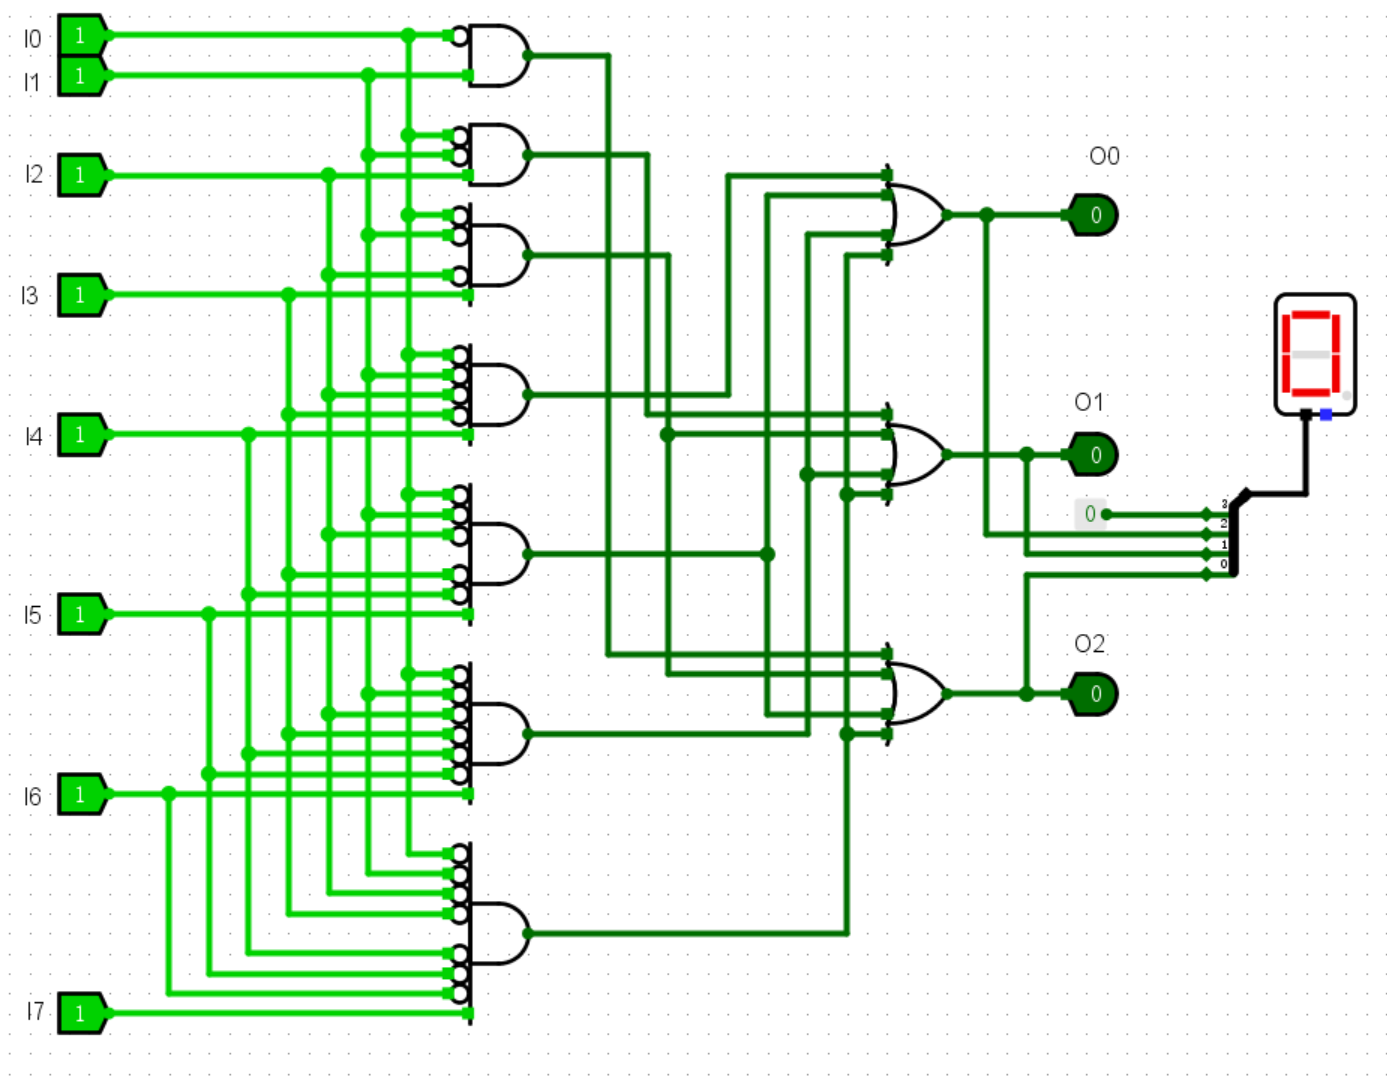
\includegraphics[width=0.4\textwidth]{2.5.1.png}
    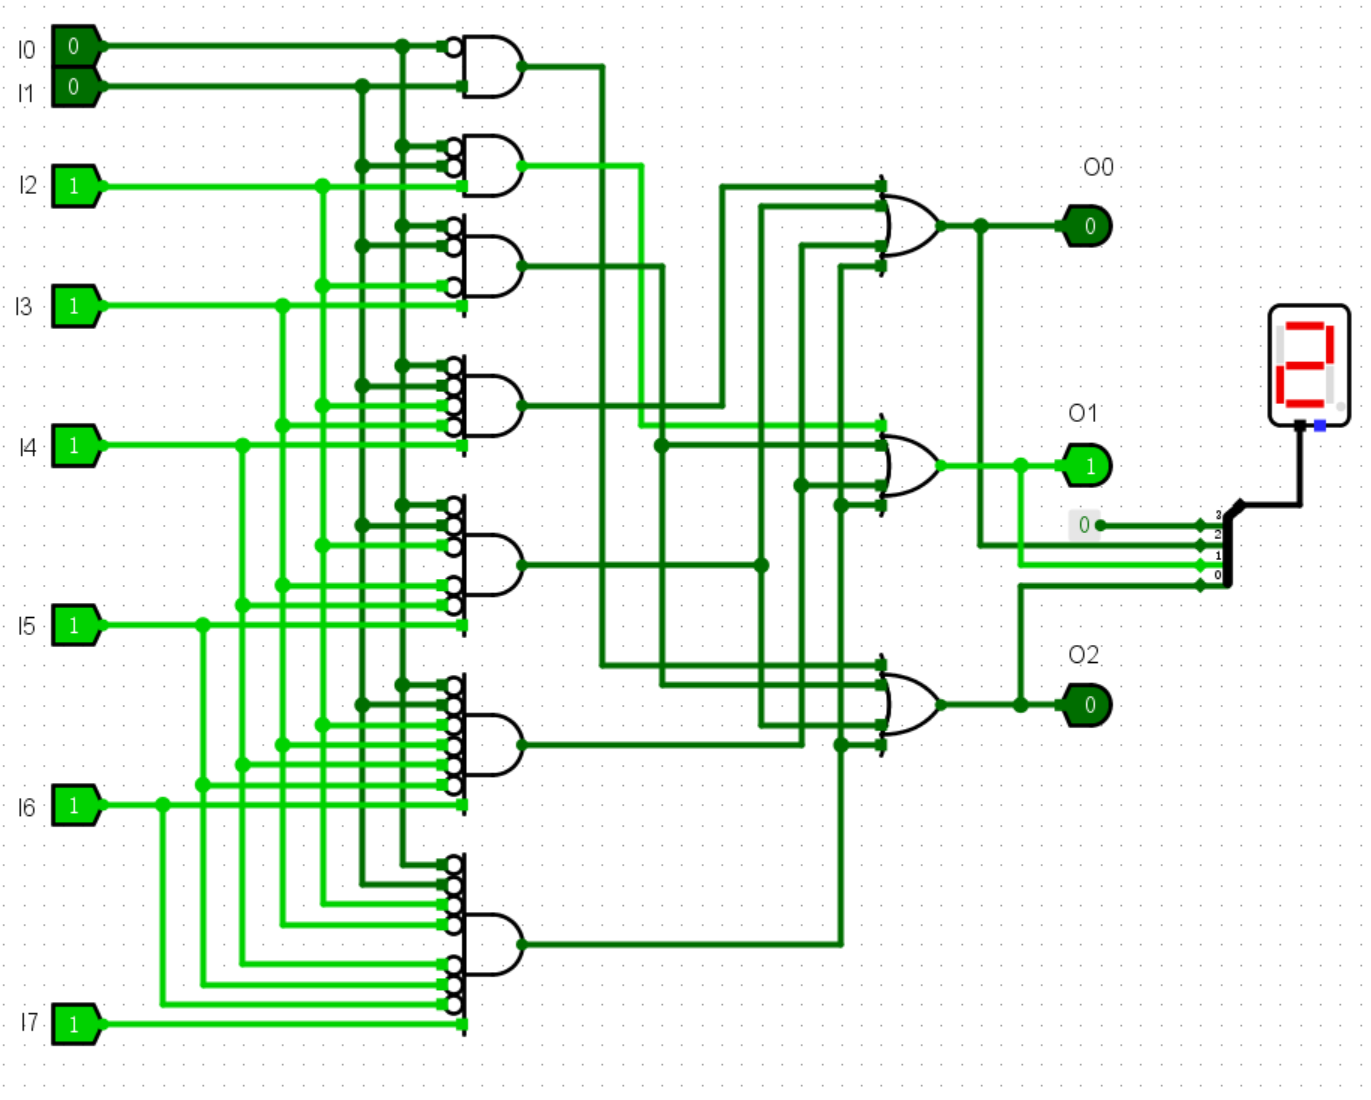
\includegraphics[width=0.4\textwidth]{2.5.2.png}
    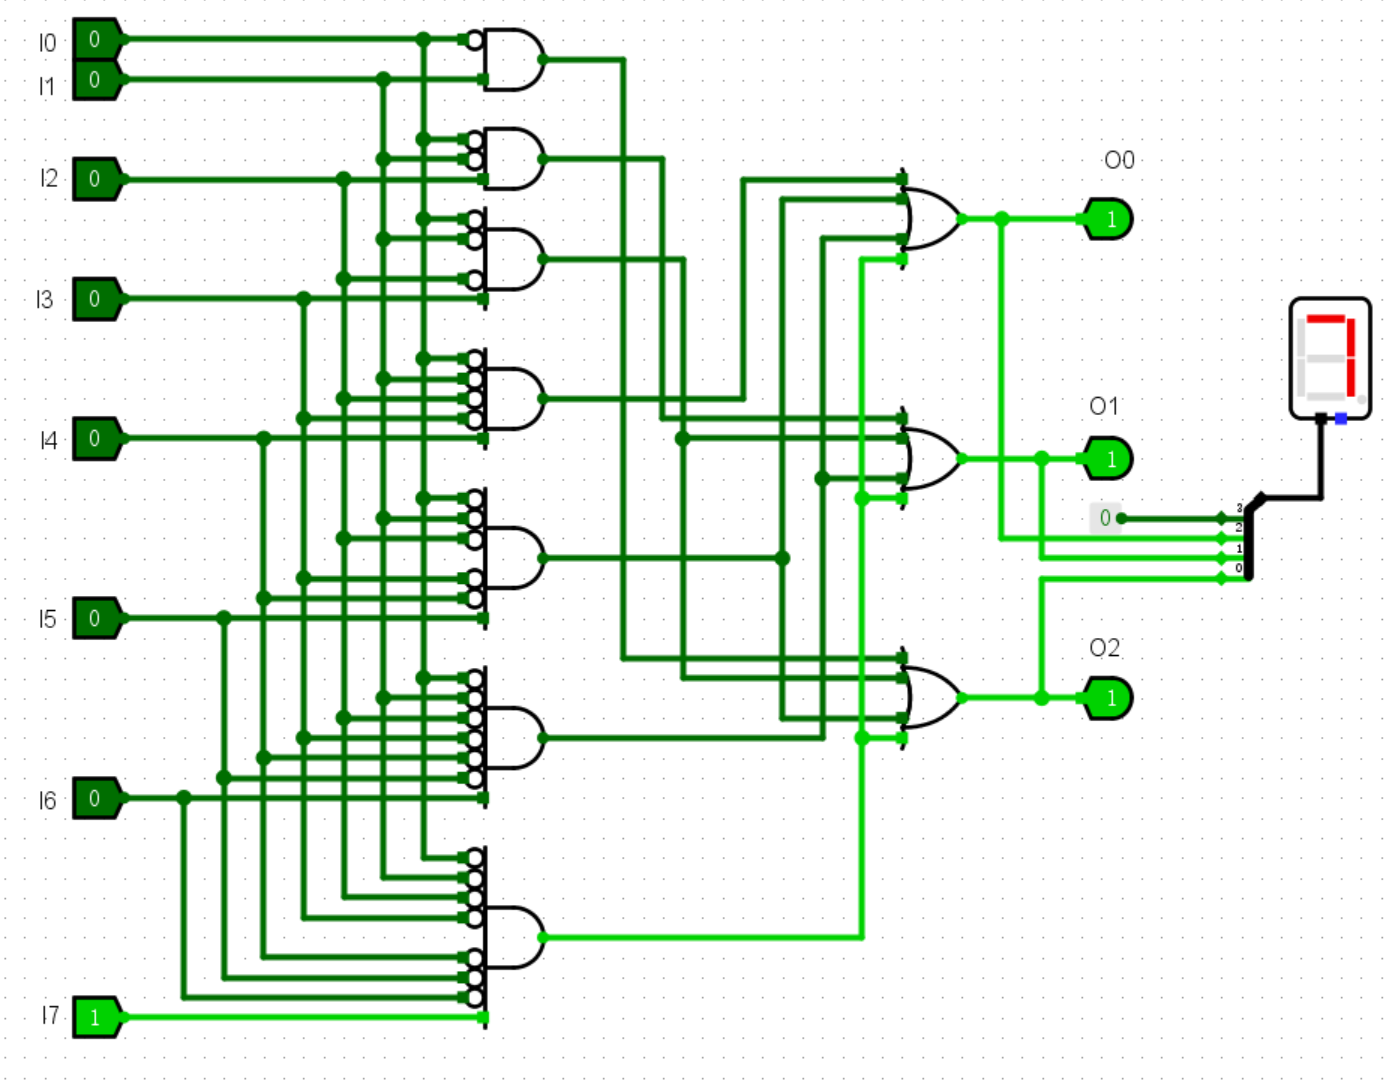
\includegraphics[width=0.4\textwidth]{2.5.3.png}
    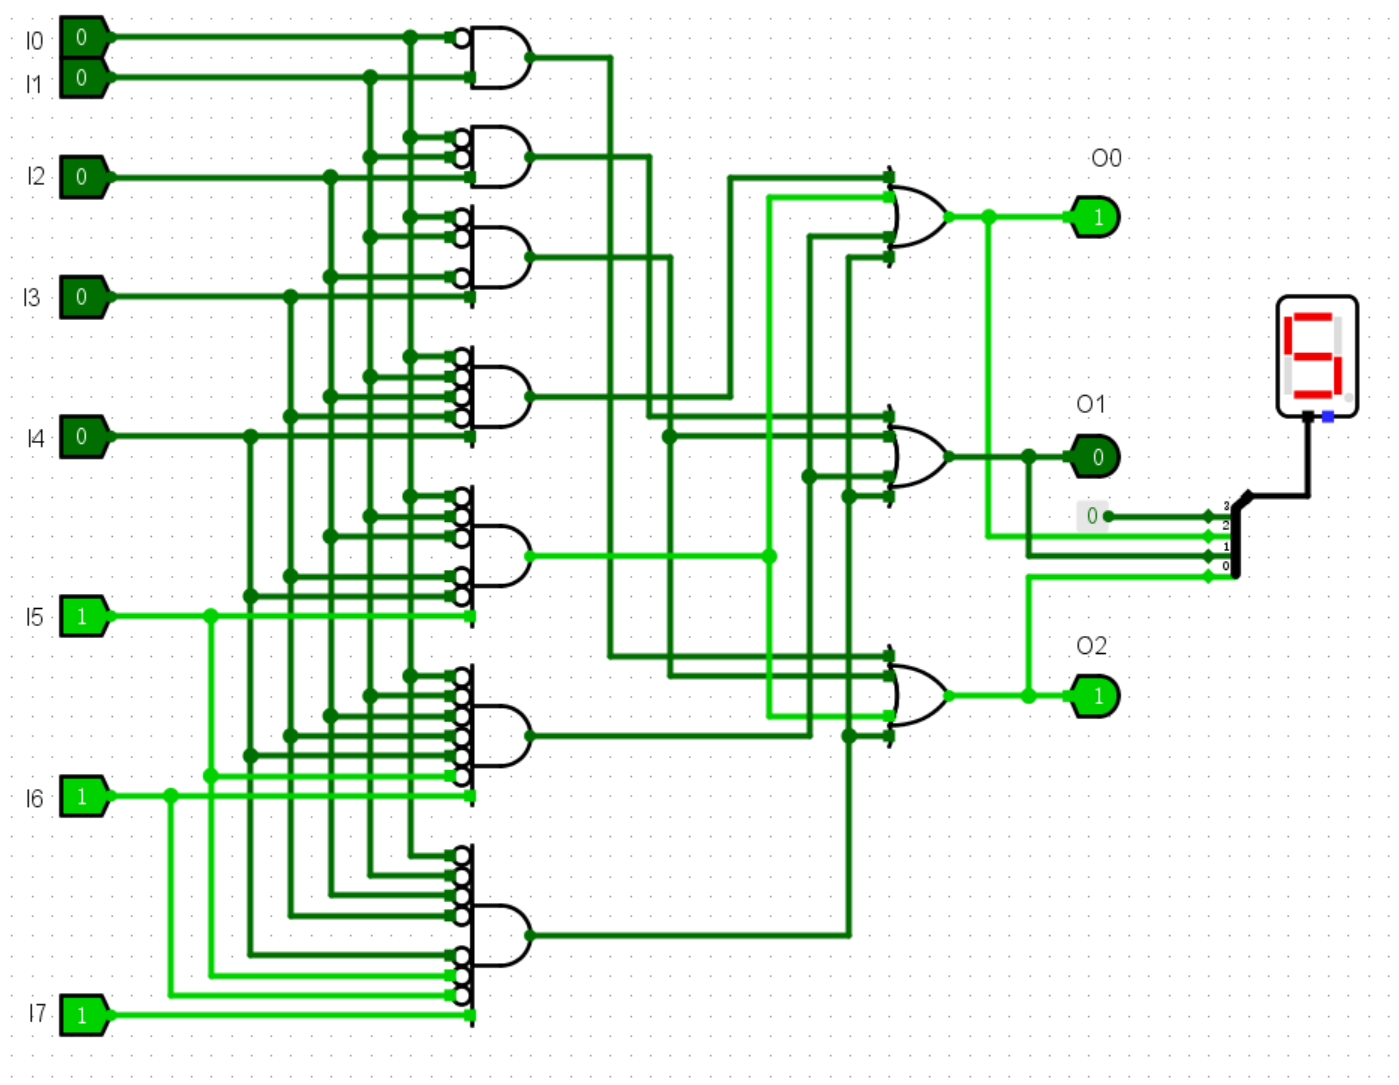
\includegraphics[width=0.4\textwidth]{2.5.4.png}
    \caption{8-3优先级编码器仿真测试}
    \end{figure}
    模拟测试如下:\\
    $I_{0}$到$I_{7}$均为1,HEX输出0。\\
    $I_2$到$I_7$均为1,其余为0,HEX输出2。\\
    $I_7$为1,其余为0,HEX输出7。\\
    $I_5$和$I_7$为1,其余为0,HEX输出5。\\

    \begin{table}[H]
    \centering
    \begin{tabular}{|c|c c|}
        \hline
        输入 & 输 & 出 \\ \hline
        $I_{0}$ $I_{1}$ $I_{2}$ $I_{3}$ $I_{4}$ $I_{5}$ $I_{6}$ $I_{7}$ & $O_{2}$ $O_{1}$ $O_{0}$ & Hex显示 \\ \hline
        1 x x x x x x x & 0 0 0 & 0 \\ \hline
        0 1 x x x x x x & 0 0 1 & 1 \\ \hline
        0 0 1 x x x x x & 0 1 0 & 2 \\ \hline
        0 0 0 1 x x x x & 0 1 1 & 3 \\ \hline
        0 0 0 0 1 x x x & 1 0 0 & 4 \\ \hline
        0 0 0 0 0 1 x x & 1 0 1 & 5 \\ \hline
        0 0 0 0 0 0 1 x & 1 1 0 & 6 \\ \hline
        0 0 0 0 0 0 0 1 & 1 1 1 & 7 \\ \hline
    \end{tabular}
    \caption{8-3优先级编码器功能表}
    \end{table}

    \subsubsection{错误现象及分析}
    在完成实验的过程中,没有遇到任何错误。

    \subsection{加法器实验}

    \subsubsection{整体方案设计}
    \begin{figure}[H]
    \centering
    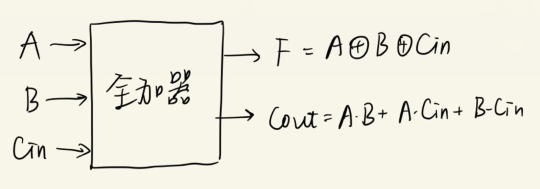
\includegraphics[width=0.8\textwidth]{3.1.png}
    \caption{全加器整体方案设计}
    \end{figure}
    
    \subsubsection{顶层模块设计}
    实验电路较为简单,不需要顶层模块设计图。

    \subsubsection{引脚作用}
    \begin{table}[H]
    \centering
    \begin{tabular}{|c|c|}
        \hline
        A\ B\ Cin & 输入引脚 \\ \hline
        F\ Cout  & 输出引脚 \\ \hline
    \end{tabular}
    \caption{全加器引脚作用}
    \end{table}

    \subsubsection{原理图和电路图}
    \begin{figure}[H]
    \centering
    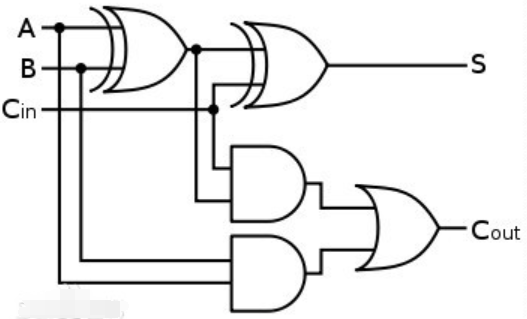
\includegraphics[width=0.8\textwidth]{3.4.1.png}
    \caption{全加器原理图}
    \end{figure}

    \begin{figure}[H]
    \centering
    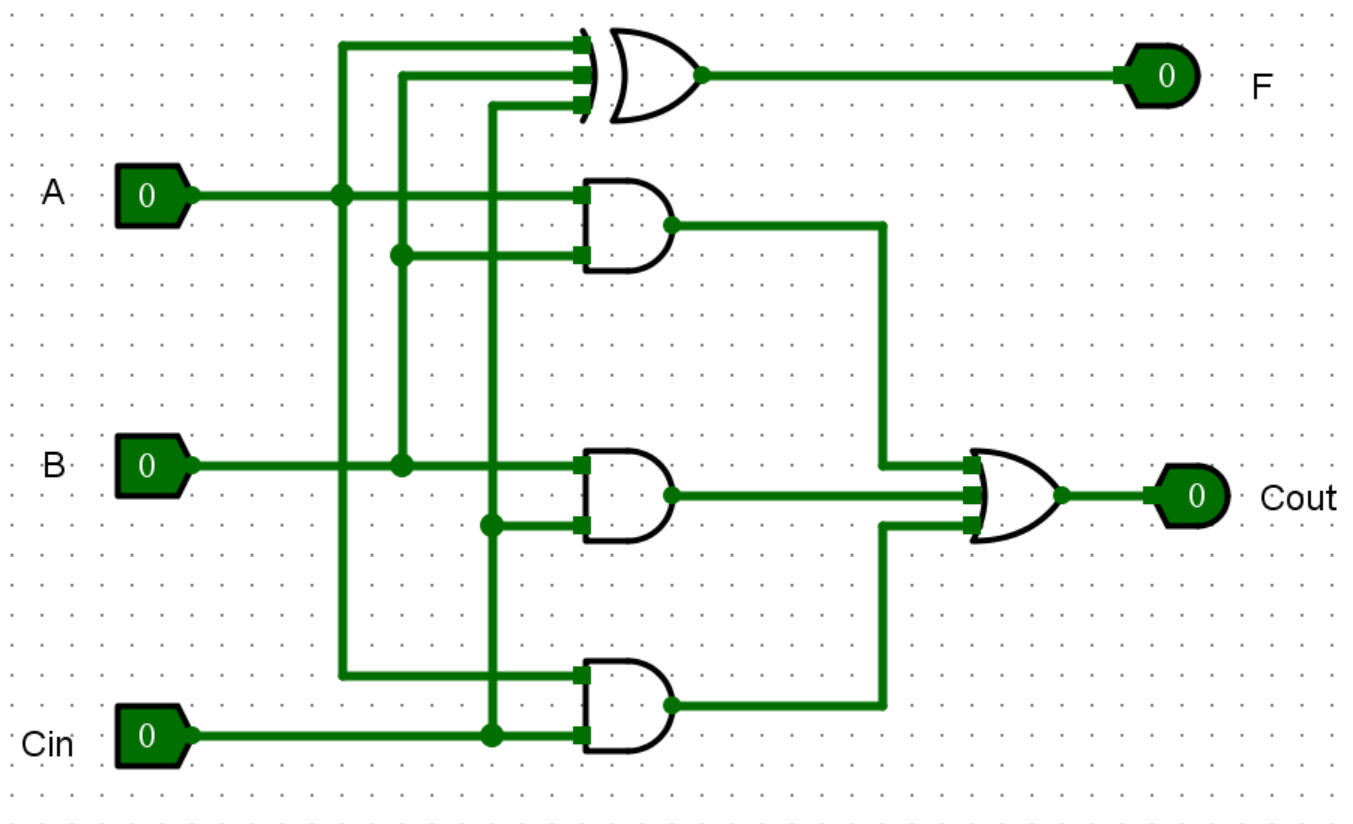
\includegraphics[width=0.8\textwidth]{3.4.2.png}
    \caption{全加器电路图}
    \end{figure}

    \subsubsection{仿真测试图}
    \begin{figure}[H]
    \centering
    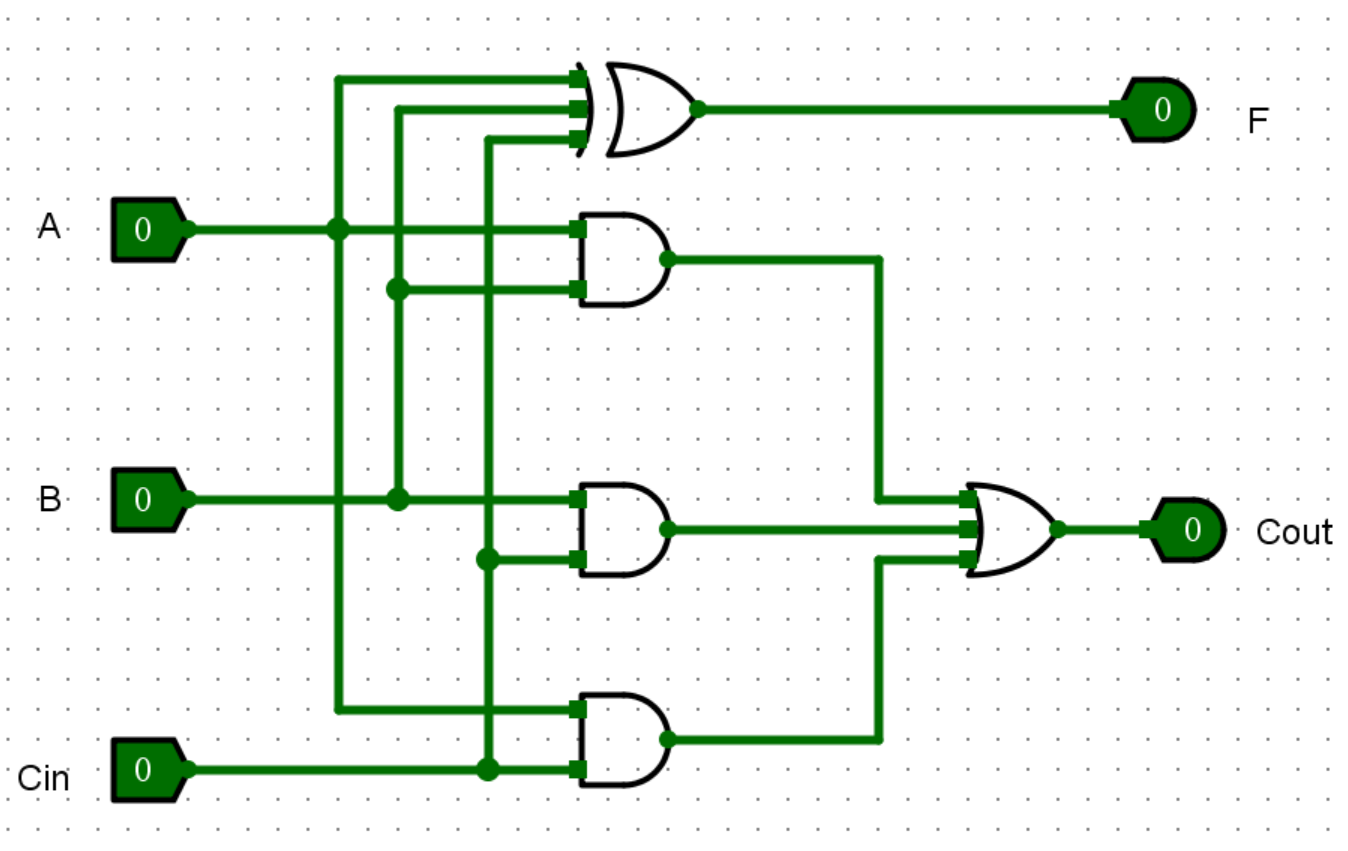
\includegraphics[width=0.4\textwidth]{3.5.1.png}
    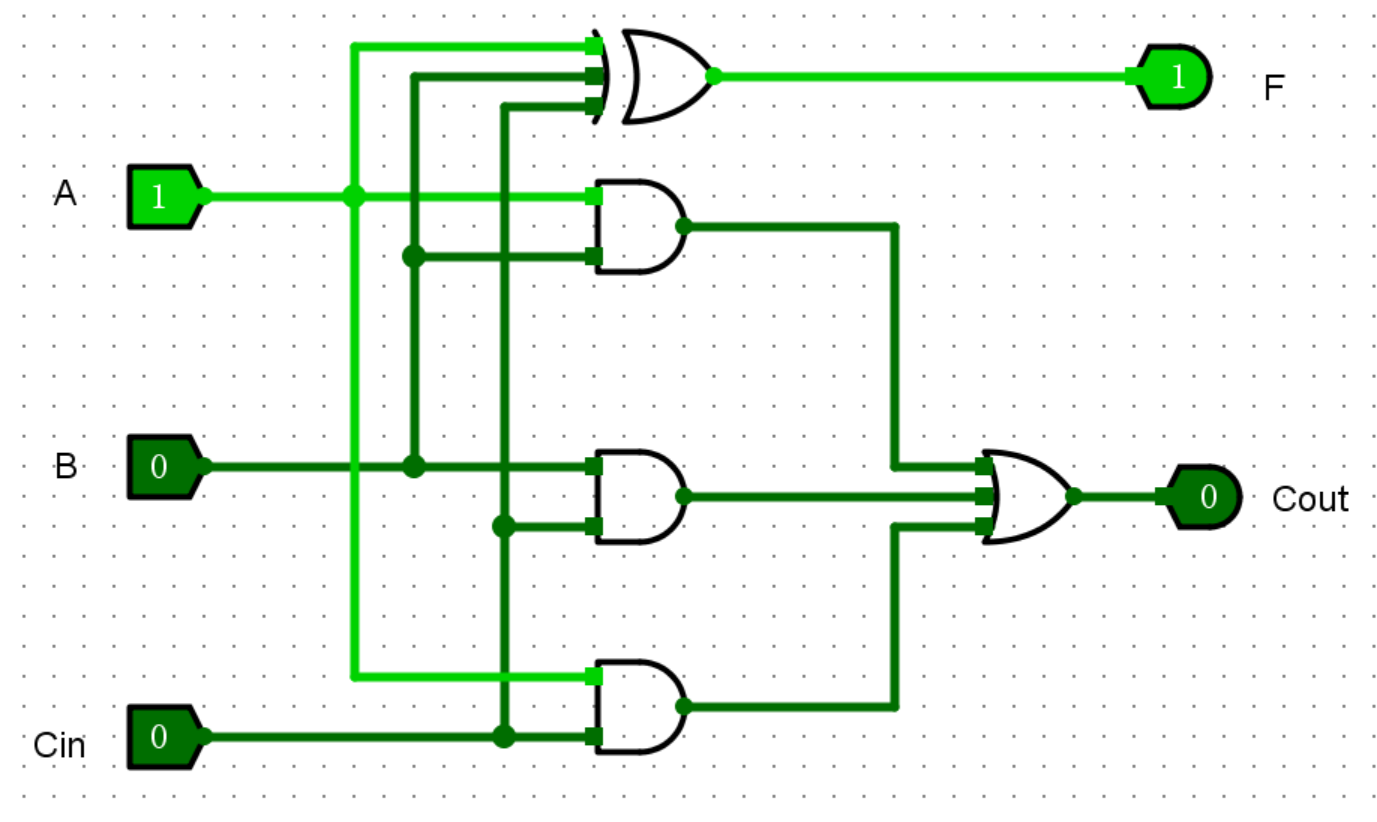
\includegraphics[width=0.4\textwidth]{3.5.2.png}
    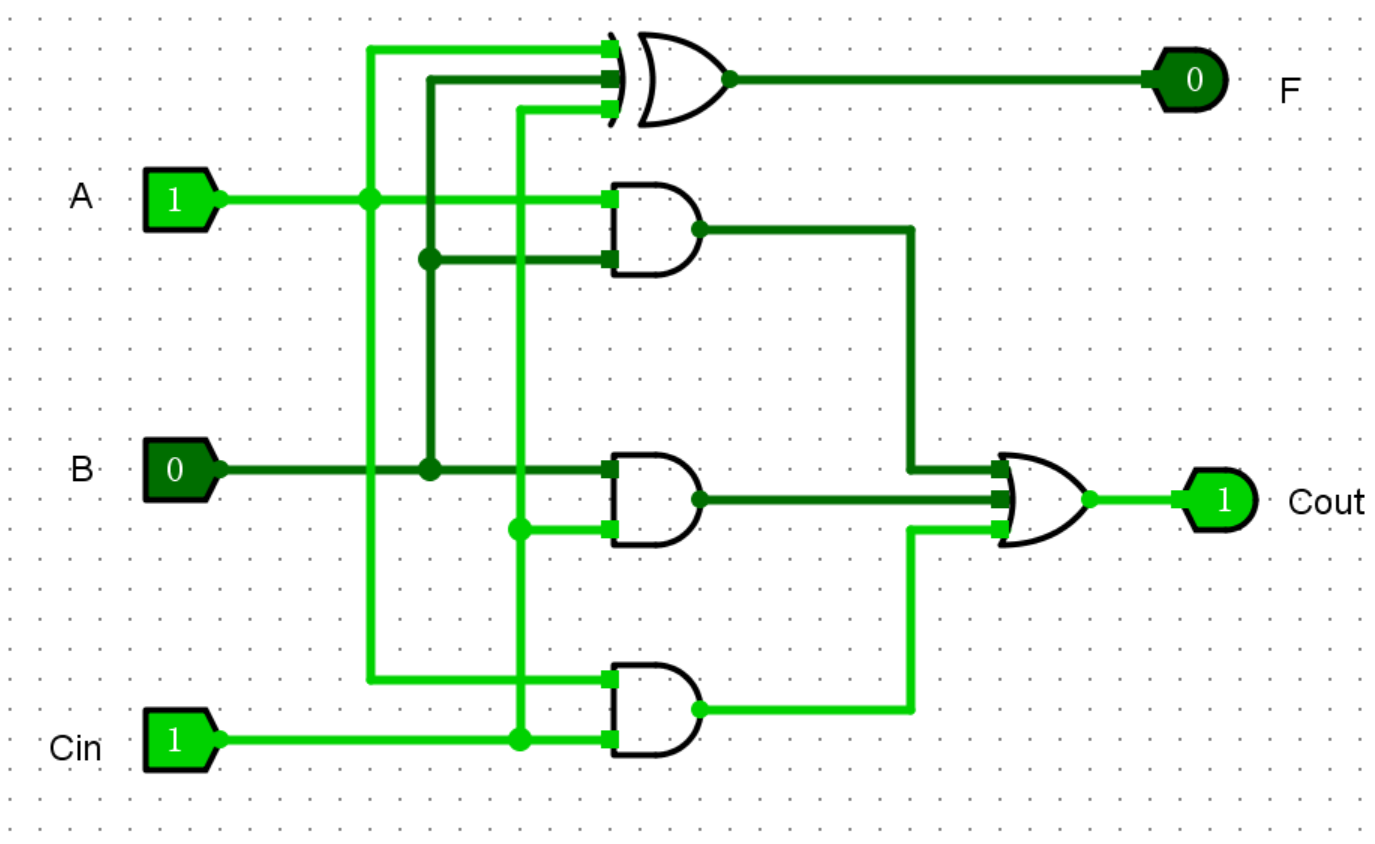
\includegraphics[width=0.4\textwidth]{3.5.3.png}
    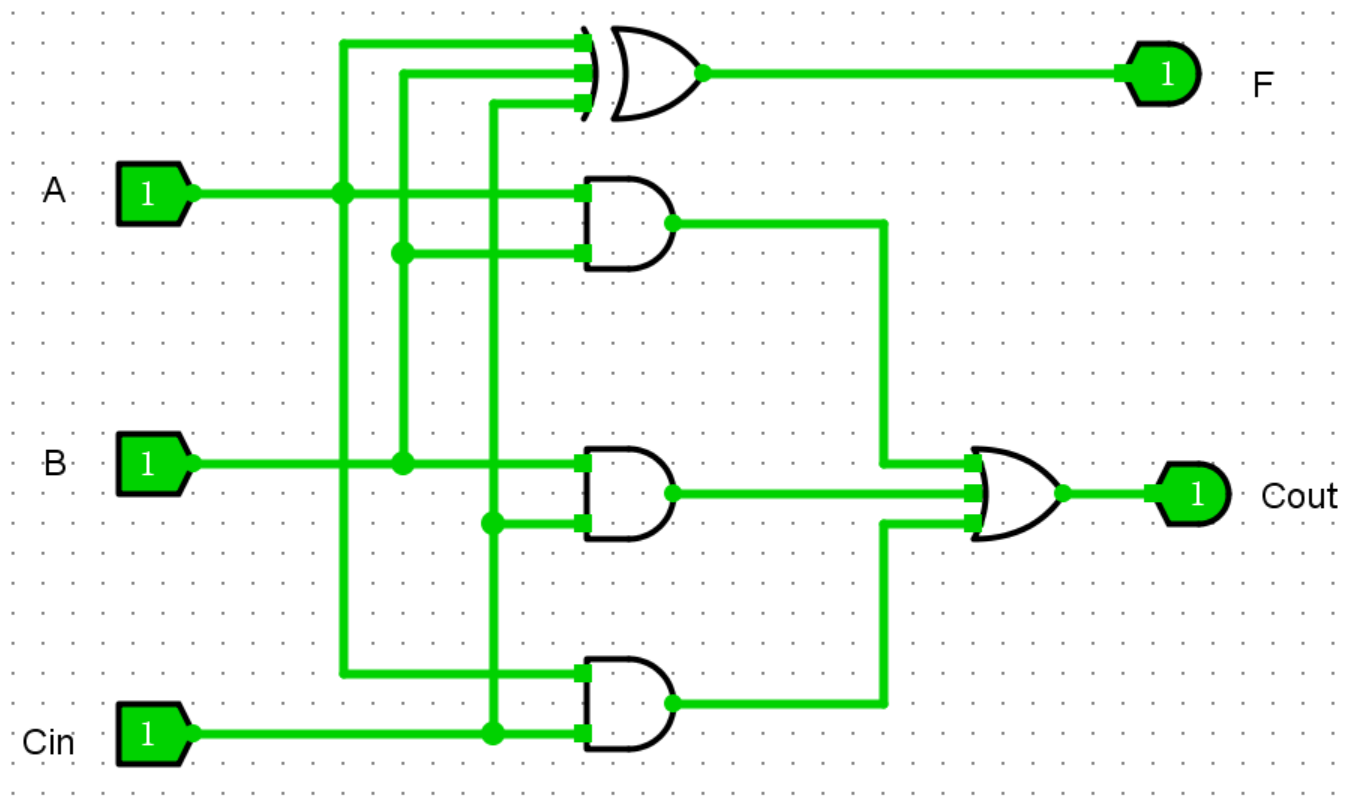
\includegraphics[width=0.4\textwidth]{3.5.4.png}
    \caption{全加器仿真测试图}
    \end{figure}


    \begin{table}[H]
    \centering
    \begin{tabular}{|c c c|c c|}
        \hline
        A & B & Cin & F & Cout \\ \hline
        0 & 0 & 0 & 0 & 0 \\ \hline
        0 & 0 & 1 & 1 & 0 \\ \hline
        0 & 1 & 0 & 1 & 0 \\ \hline
        0 & 1 & 1 & 0 & 1 \\ \hline
        1 & 0 & 0 & 1 & 0 \\ \hline
        1 & 0 & 1 & 0 & 1 \\ \hline
        1 & 1 & 0 & 0 & 1 \\ \hline
        1 & 1 & 1 & 1 & 1 \\ \hline
    \end{tabular}
    \caption{全加器真值表}
    \end{table}

    \subsubsection{错误现象及分析}
    在完成实验的过程中,没有遇到任何错误。


    \subsection{4位串行进位加减法器}

    \subsubsection{整体方案设计}
    \begin{figure}[H]
    \centering
    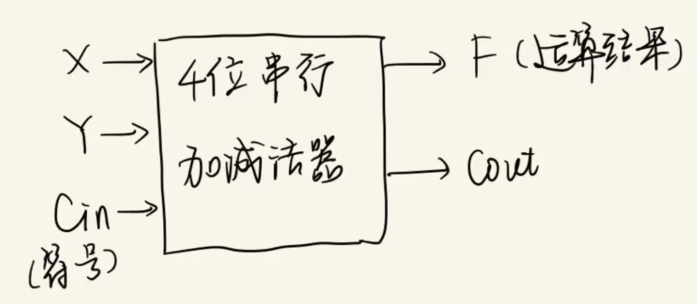
\includegraphics[width=0.8\textwidth]{4.1.png}
    \caption{4位串行进位加减法器整体方案设计}
    \end{figure}
    
    \subsubsection{顶层模块设计}
    实验电路较为简单,不需要顶层模块设计图。

    \subsubsection{引脚作用}
    \begin{table}[H]
    \centering
    \begin{tabular}{|c|c|}
        \hline
        X Y Cin & 输入引脚 \\ \hline
        F Cout & 输出引脚 \\ \hline
    \end{tabular}
    \caption{4位串行进位加减法器引脚作用}
    \end{table}

    \subsubsection{原理图和电路图}
    \begin{figure}[H]
    \centering
    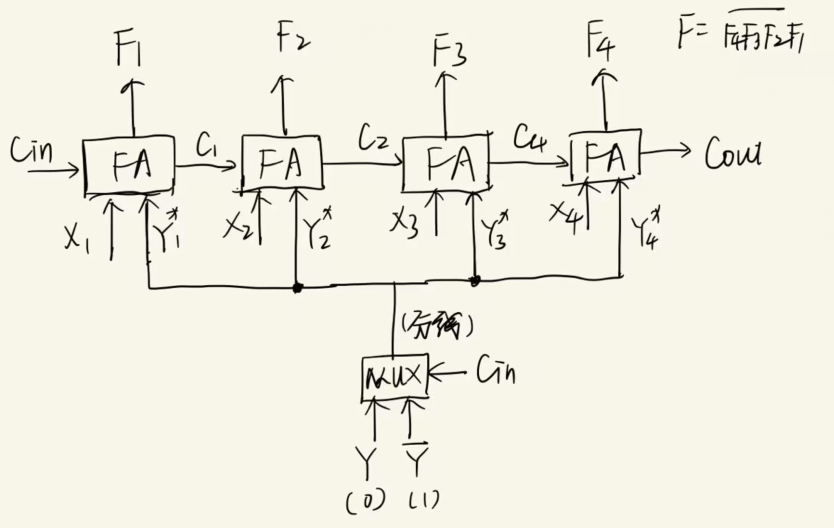
\includegraphics[width=0.8\textwidth]{4.4.1.png}
    \caption{4位串行进位加减法器原理图}
    \end{figure}

    \begin{figure}[H]
    \centering
    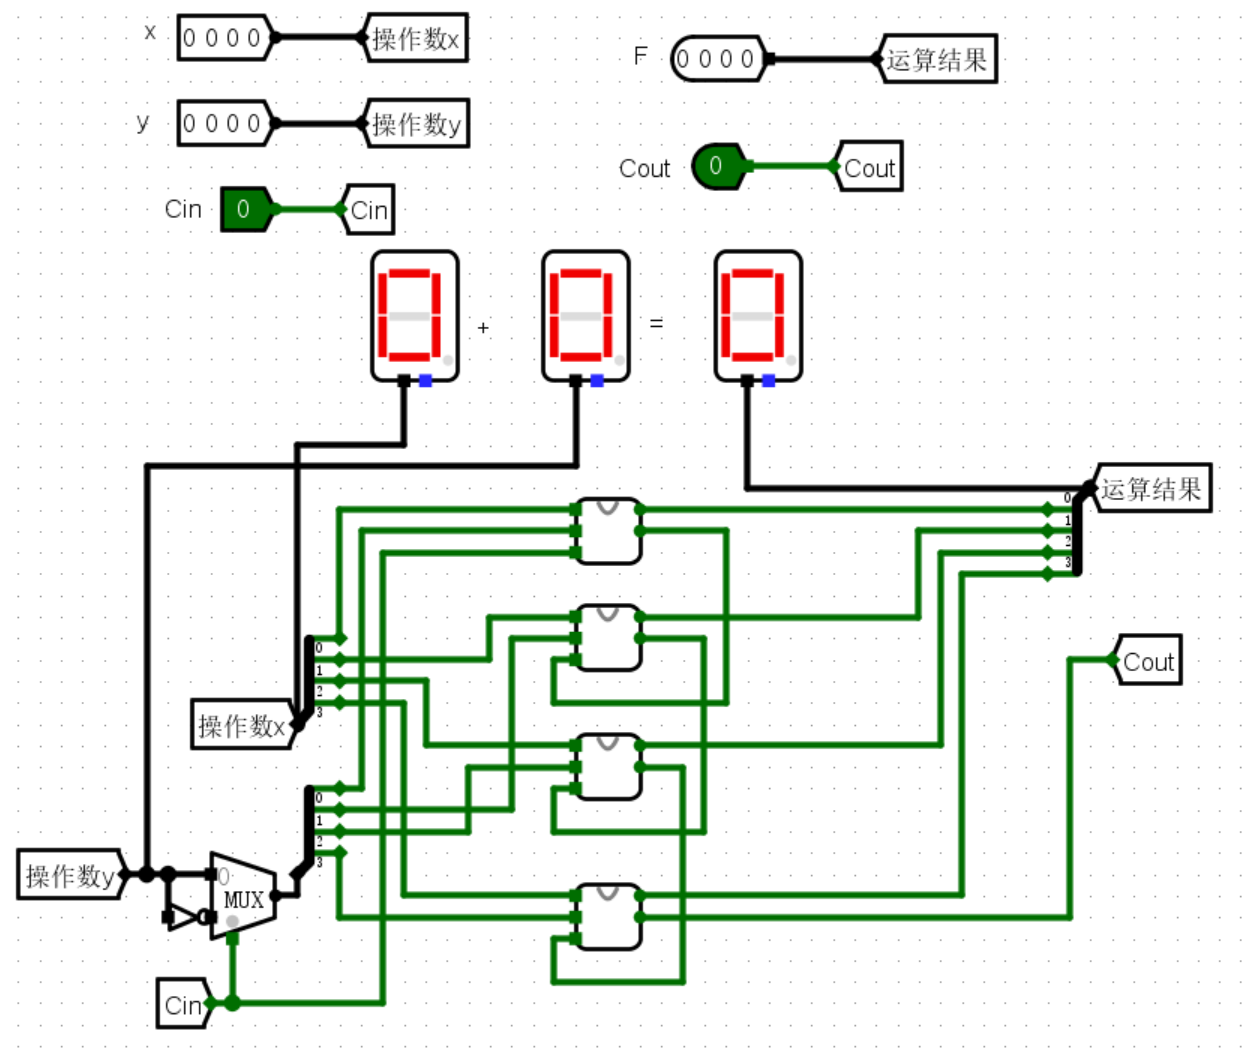
\includegraphics[width=0.8\textwidth]{4.4.2.png}
    \caption{4位串行进位加减法器电路图}
    \end{figure}

    \subsubsection{仿真测试图}
    \begin{figure}[H]
    \centering
    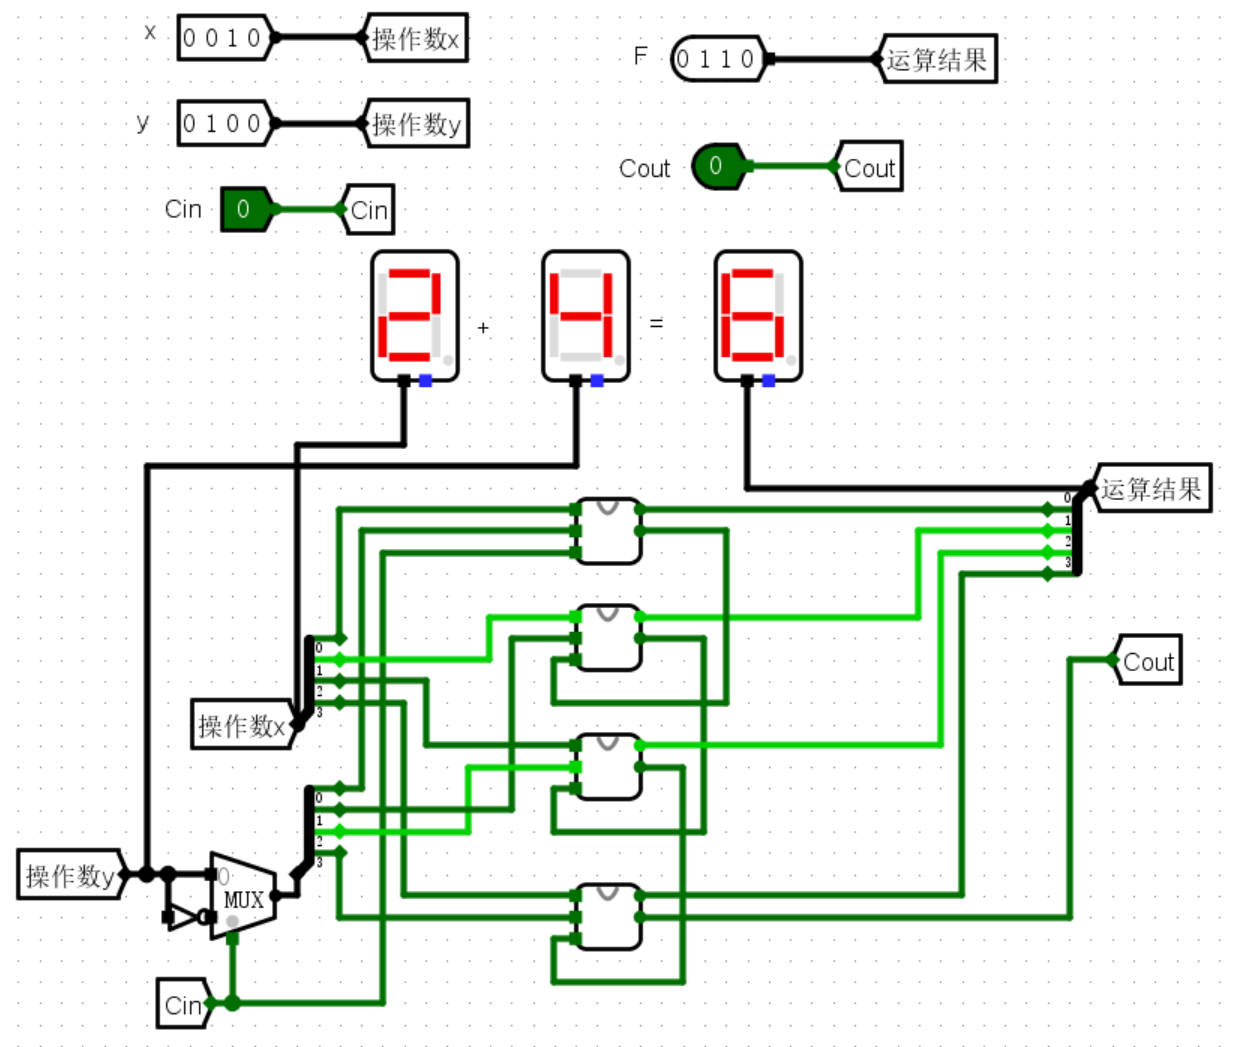
\includegraphics[width=0.4\textwidth]{4.5.1.png}
    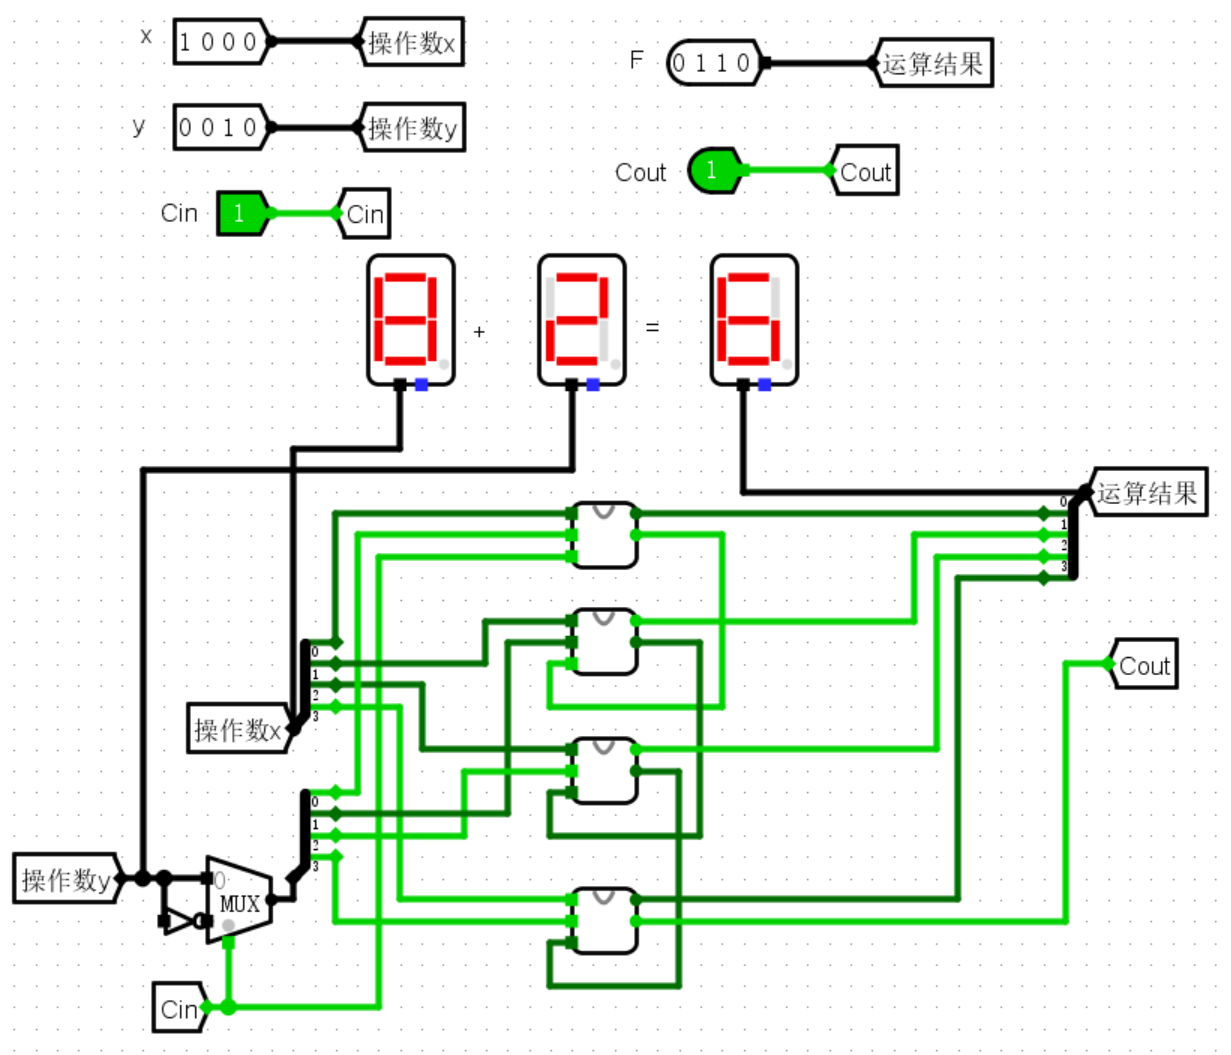
\includegraphics[width=0.4\textwidth]{4.5.2.png}
    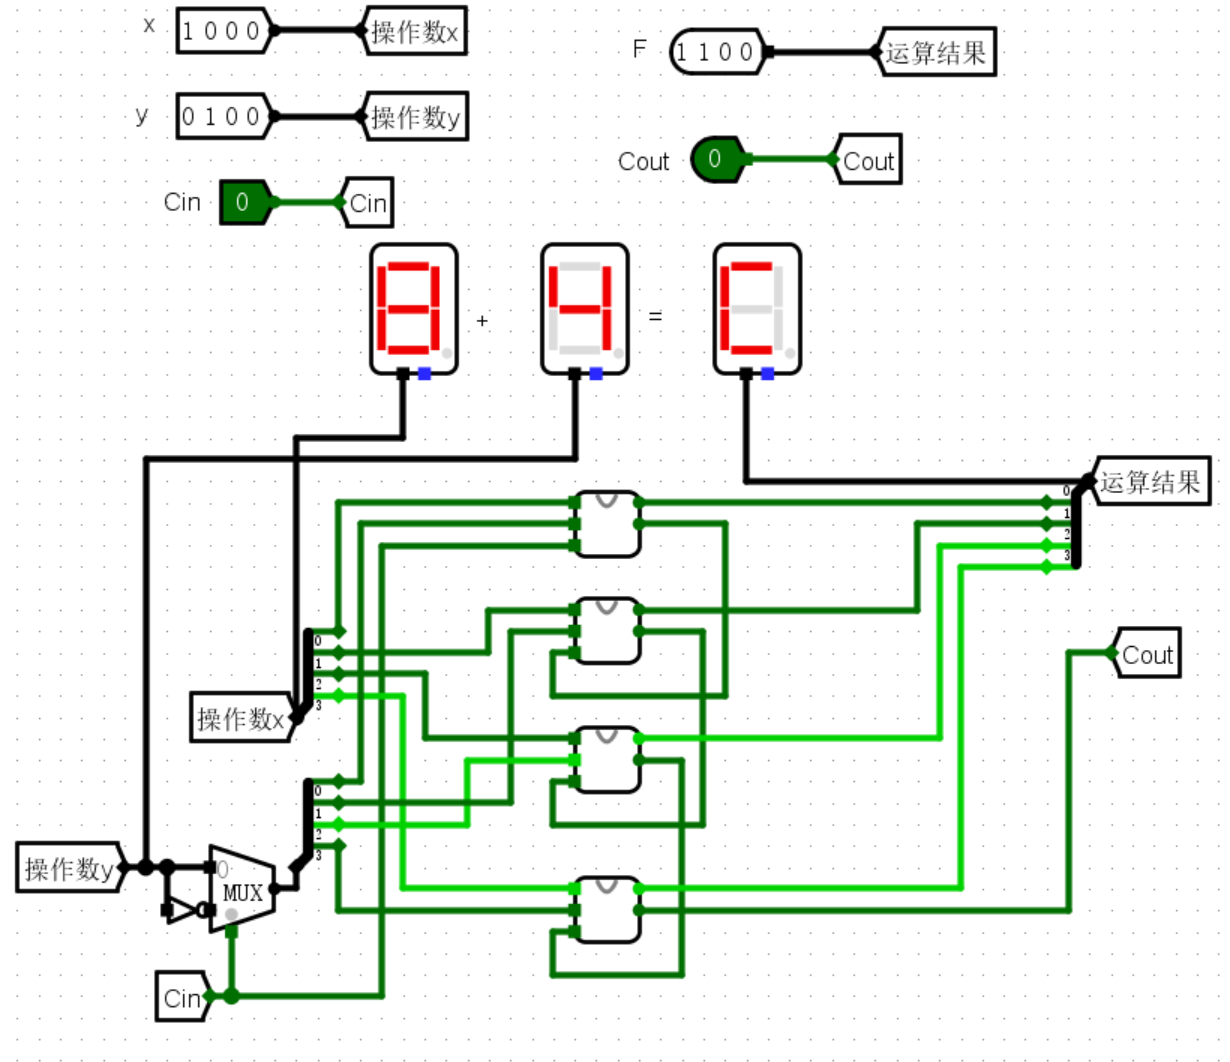
\includegraphics[width=0.4\textwidth]{4.5.3.png}
    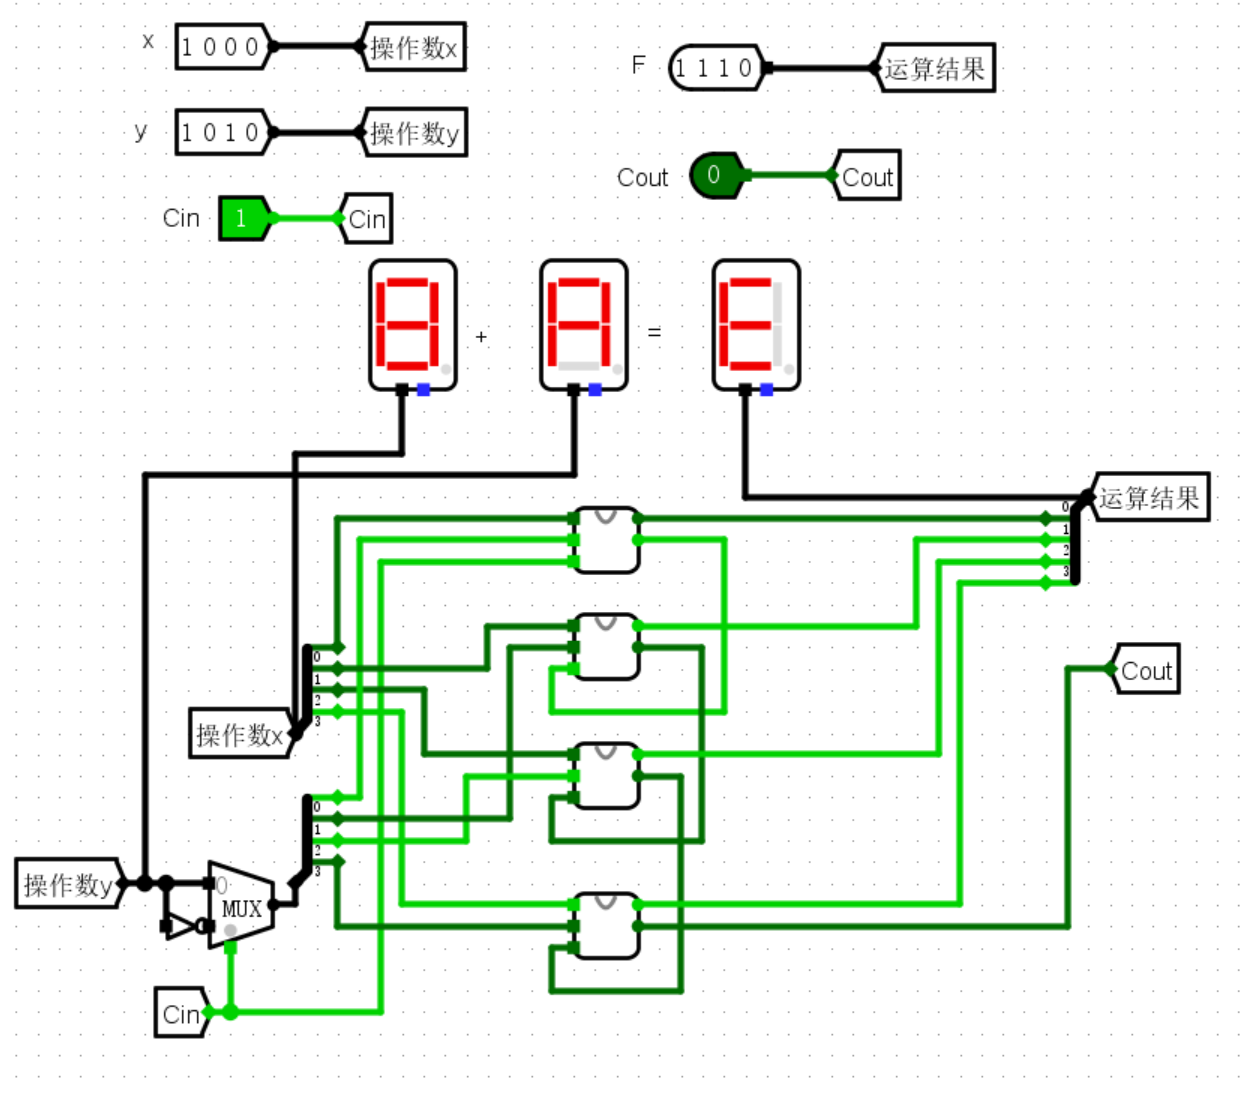
\includegraphics[width=0.4\textwidth]{4.5.4.png}
    \caption{4位串行进位加减法器仿真测试图}
    \end{figure}
    仿真测试如下:\\
    图一X为2,Y为4,Cin为0,输出F为6,Cout为0。\\
    图二X为8,Y为2,Cin为1,输出F为6,Cout为1。\\
    图三X为8,Y为4,Cin为0,输出F为C,Cout为0。\\
    图四X为8,Y为A,Cin为1,输出F为E,Cout为0。

    \begin{table}[H]
    \centering
    \begin{tabular}{|c|c|c|c|}
        \hline
        Cin & F & Cout & 功能 \\ \hline
        0 & X+Y & 0 & 加法器且未溢出 \\ \hline
        0 & X+Y & 1 & 加法器且溢出 \\ \hline
        1 & X-Y & 0 & 减法器且未溢出 \\ \hline
        1 & X-Y & 1 & 减法器且溢出 \\ \hline
    \end{tabular}
    \caption{4位串行进位加减法器功能表}
    \end{table}

    \subsubsection{错误现象及分析}
    在完成实验的过程中,没有遇到任何错误。

    \subsection{汉明码校验电路}

    \subsubsection{整体方案设计}
    \begin{figure}[H]
    \centering
    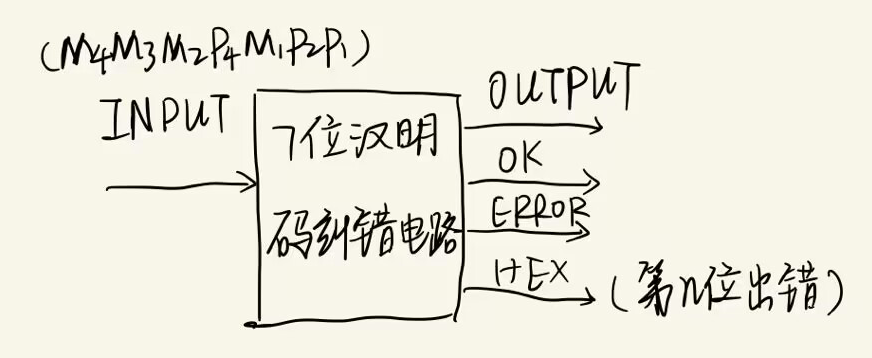
\includegraphics[width=0.8\textwidth]{5.1.png}
    \caption{汉明码校验电路整体方案设计}
    \end{figure}
    
    \subsubsection{顶层模块设计}
    实验电路较为简单,不需要顶层模块设计图。

    \subsubsection{引脚作用}
    \begin{table}[H]
    \centering
    \begin{tabular}{|c|c|}
        \hline
        X & 输入引脚 \\ \hline
        F OK Error HEX & 输出引脚 \\ \hline
    \end{tabular}
    \caption{汉明码校验电路引脚作用}
    \end{table}

    \subsubsection{原理图和电路图}
    \begin{figure}[H]
    \centering
    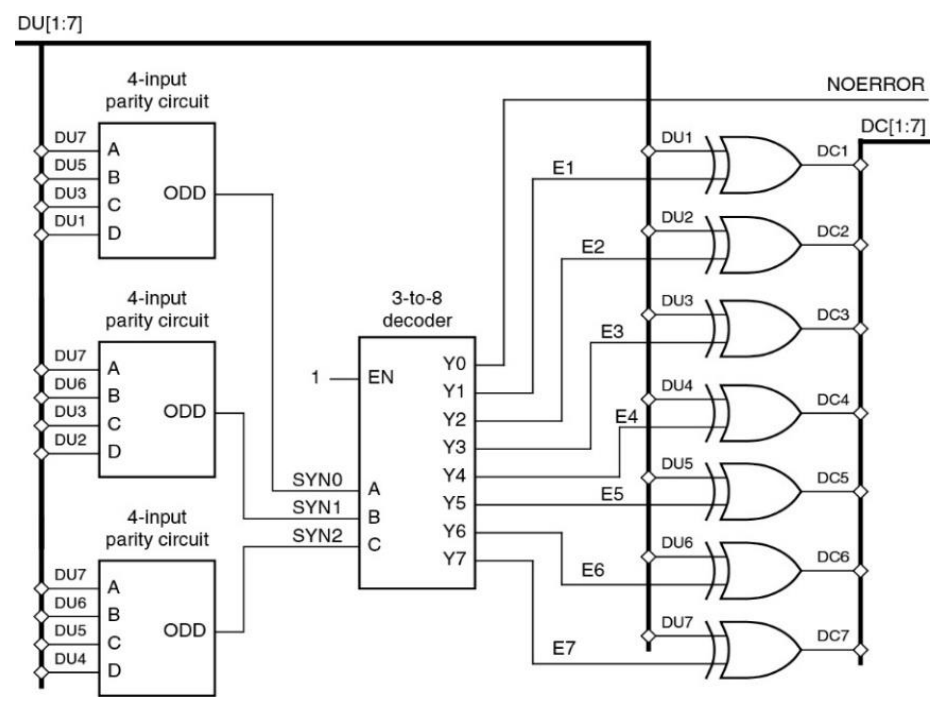
\includegraphics[width=0.8\textwidth]{5.4.1.png}
    \caption{汉明码校验电路原理图}
    \end{figure}

    \begin{figure}[H]
    \centering
    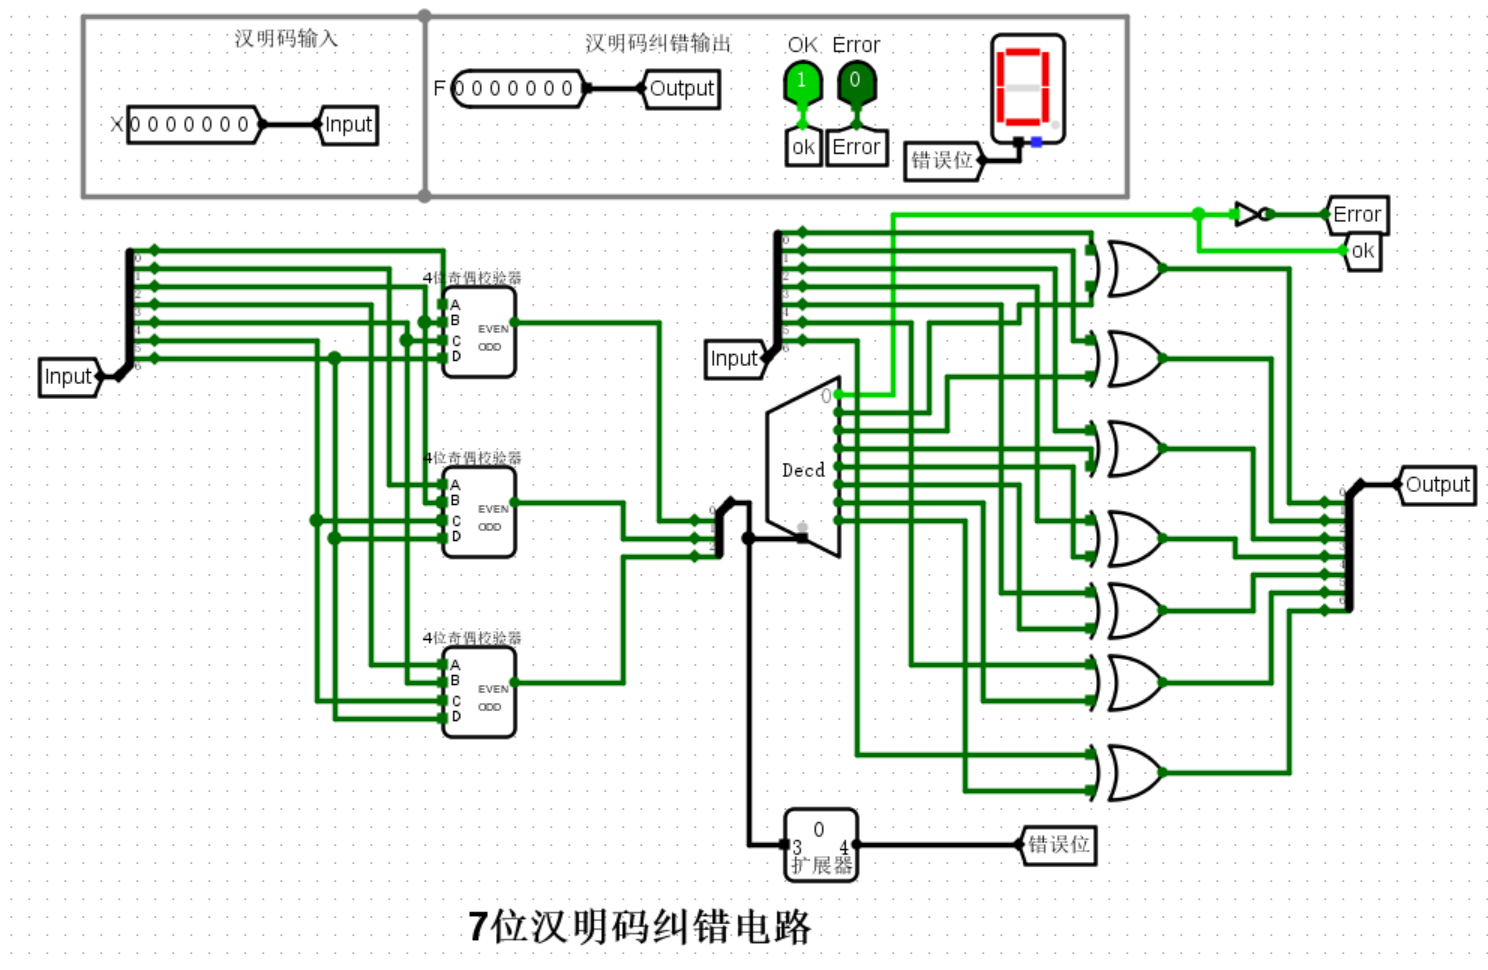
\includegraphics[width=0.8\textwidth]{5.4.2.png}
    \caption{汉明码校验电路电路图}
    \end{figure}

    \subsubsection{仿真测试图}
    \begin{figure}[H]
    \centering
    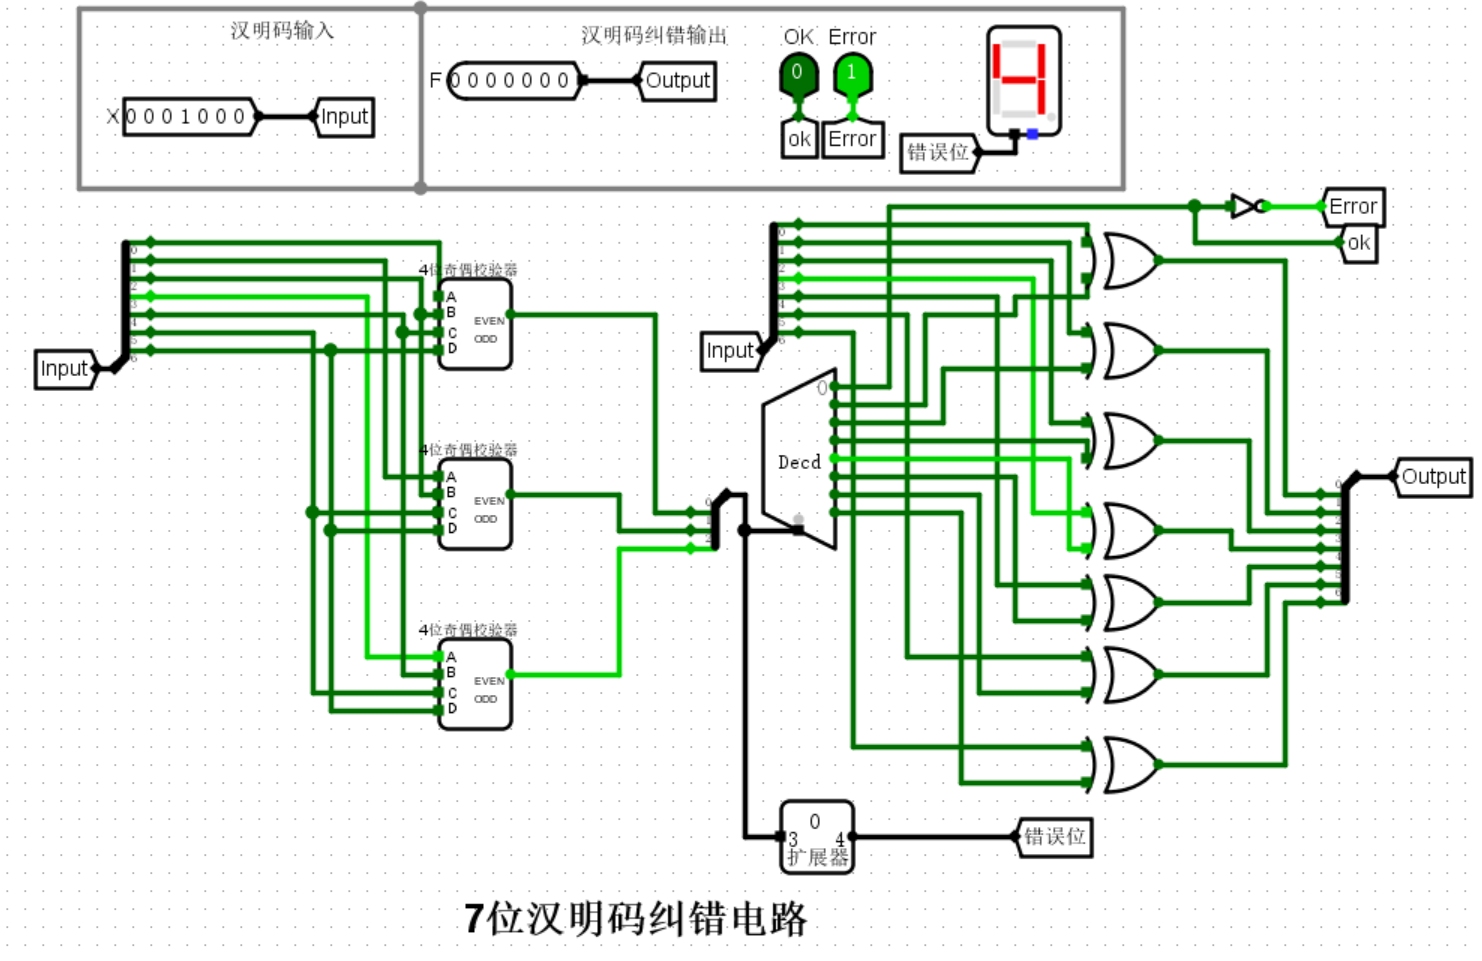
\includegraphics[width=0.4\textwidth]{5.5.1.png}
    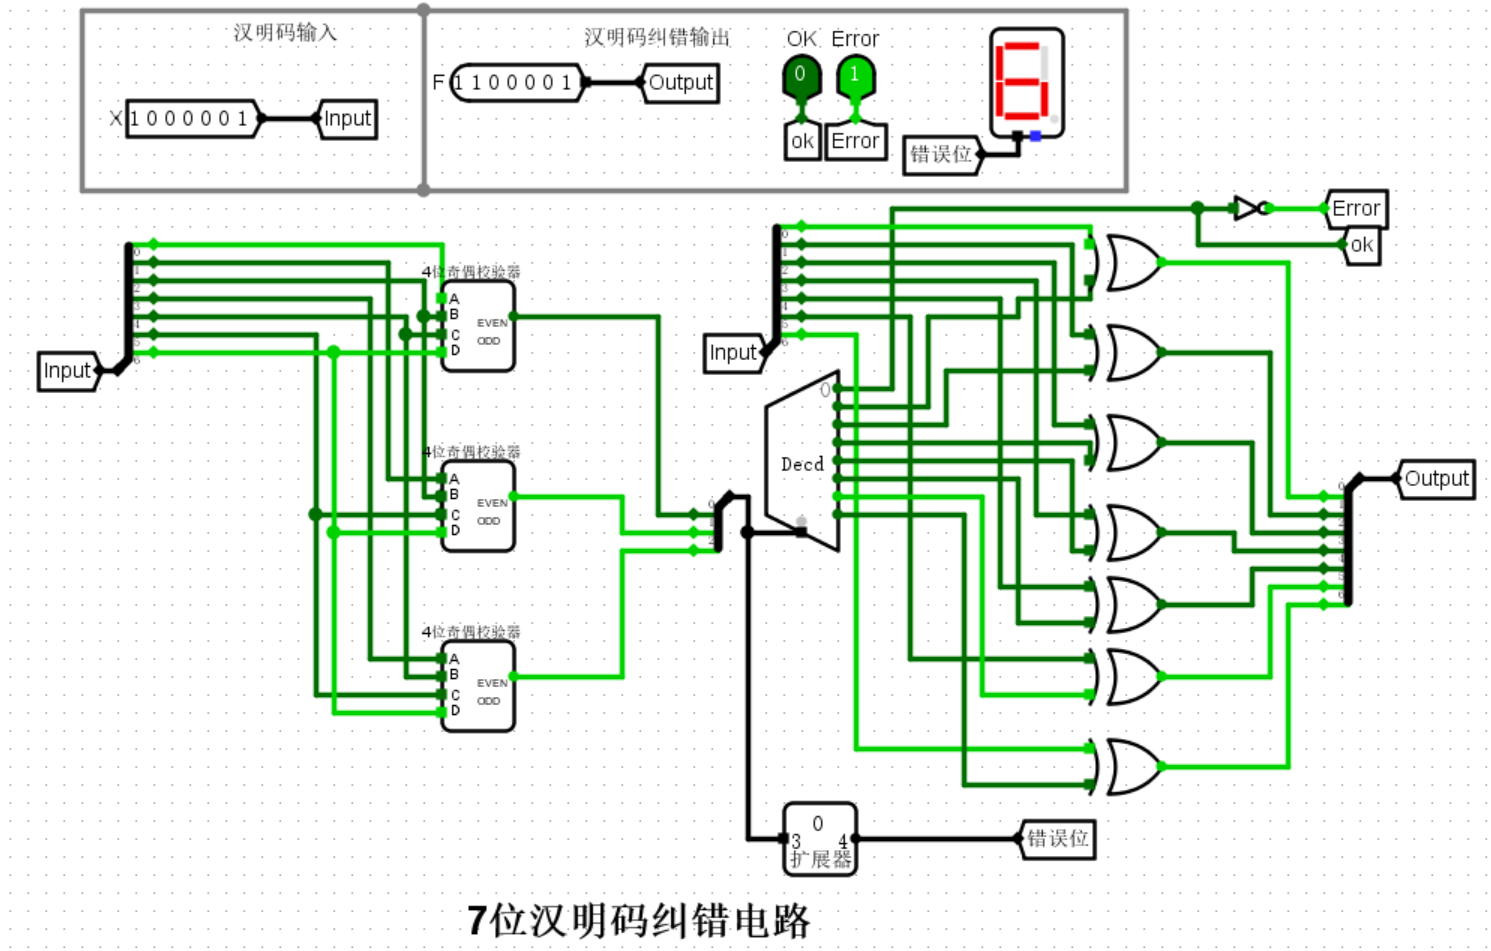
\includegraphics[width=0.4\textwidth]{5.5.2.png}
    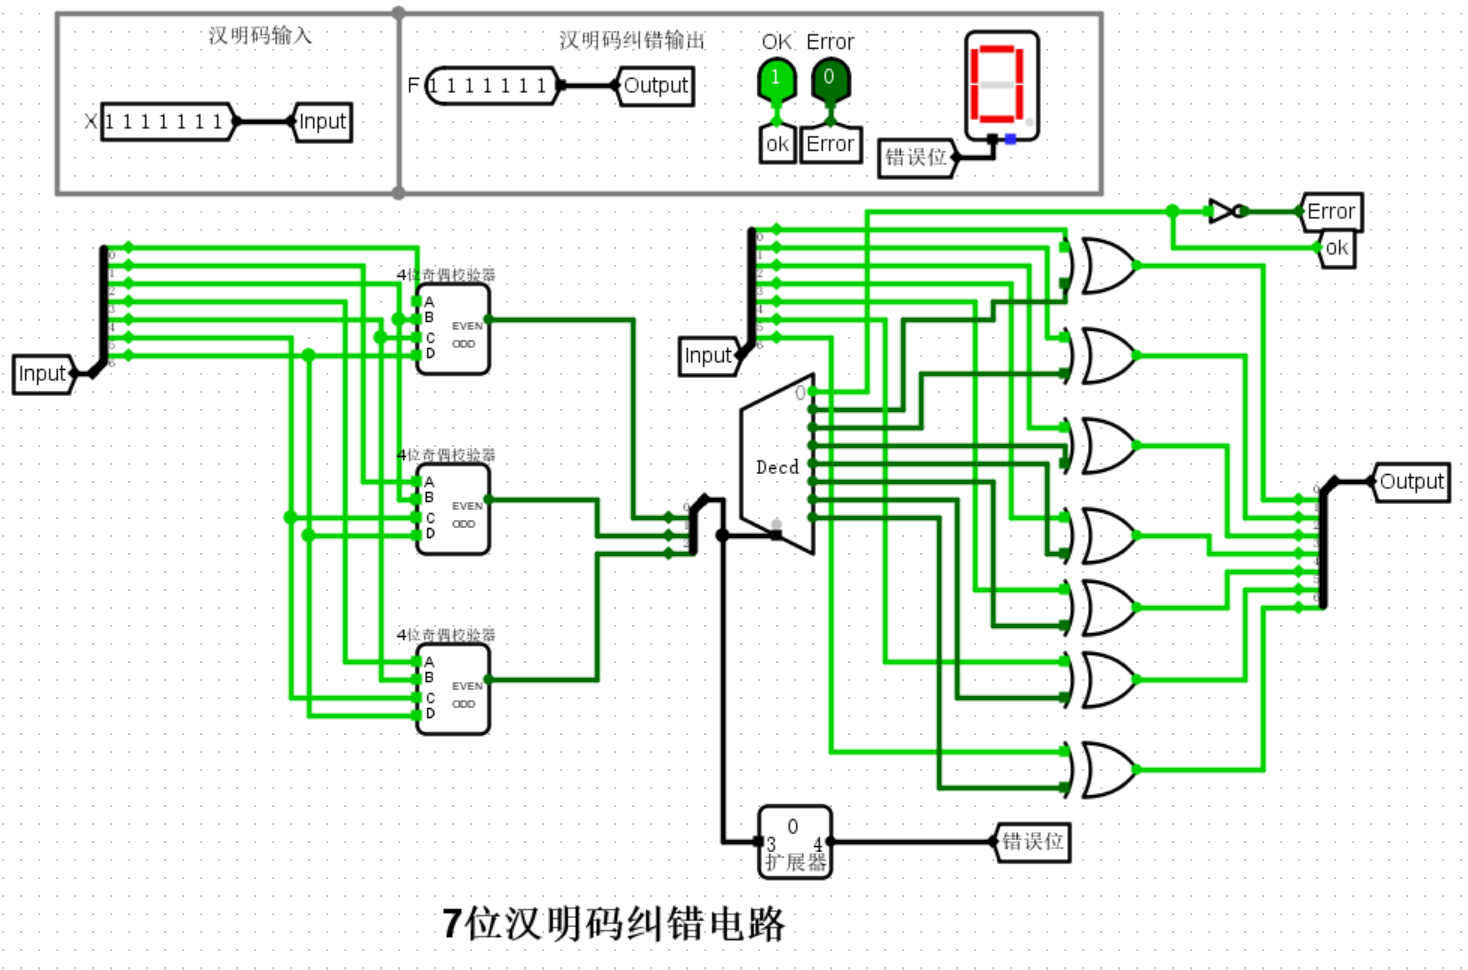
\includegraphics[width=0.4\textwidth]{5.5.3.png}
    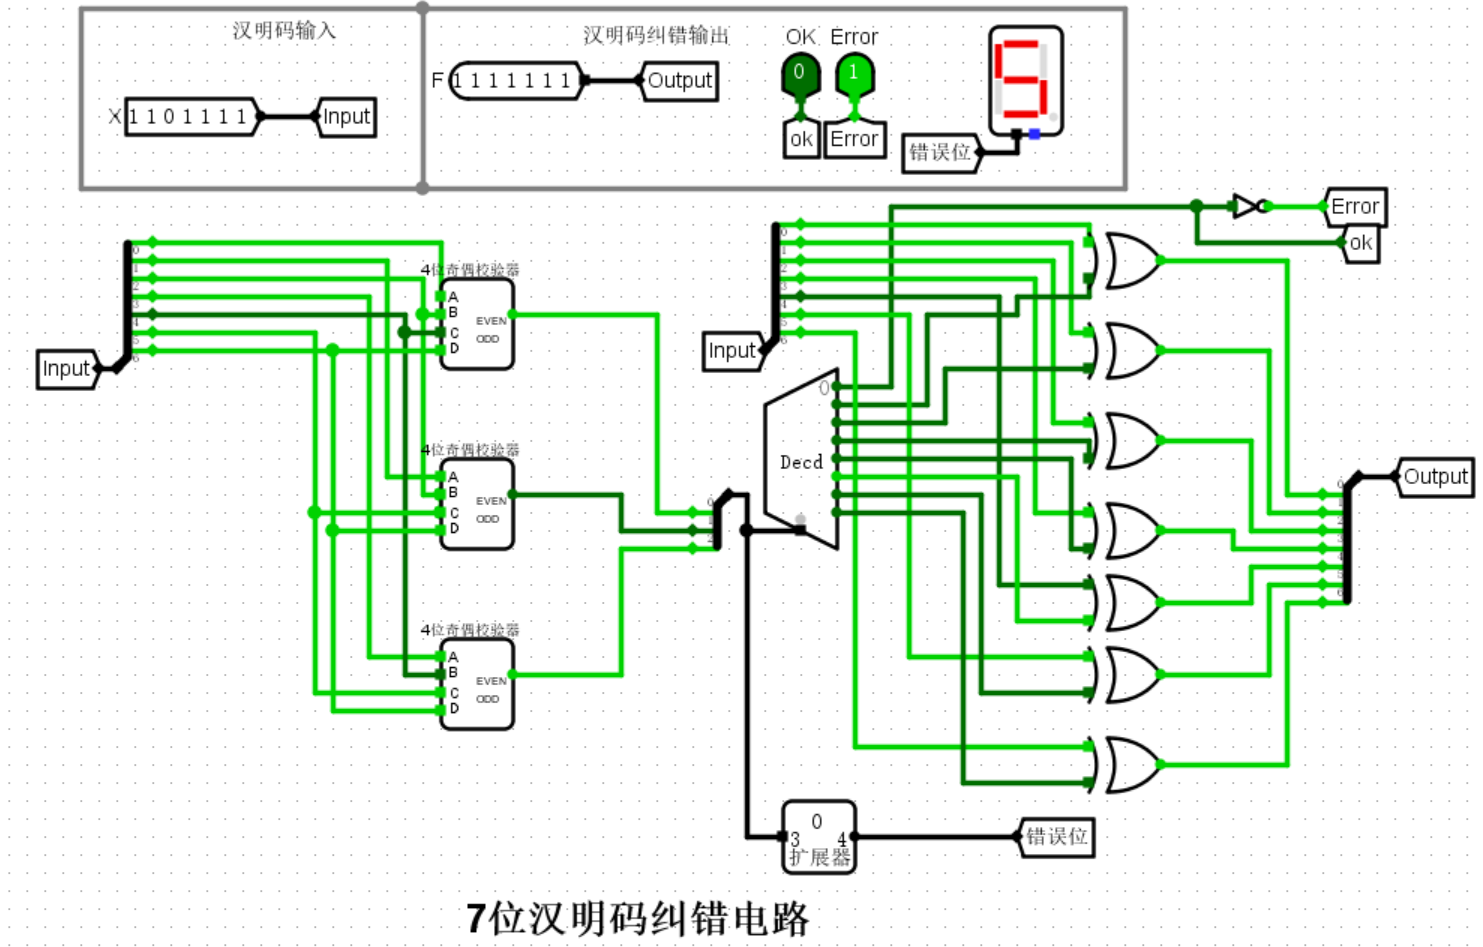
\includegraphics[width=0.4\textwidth]{5.5.4.png}
    \caption{汉明码校验电路仿真测试图}
    \end{figure}
    仿真测试如下:\\
    图一X为0001000,错误位为第4位,Error为1,OK为0,输出F为0000000。\\
    图二X为1000001,错误位为第6位,Error为1,OK为0,输出F为1100001。\\
    图三X为1111111,正确,Error为0,OK为1,输出F为1111111。\\
    图四X为1101111,错误位为第5位,Error为1,OK为0,输出F为1111111。

    \begin{table}[H]
    \centering
    \begin{tabular}{|c|c|c|c|c|c|}
        \hline
        X & F & OK & Error & HEX & 功能 \\ \hline
        Input & Output & 1 & 0 & 0 & 数据正确 \\ \hline
        Input & Output & 0 & 1 & x & 第x位错误 \\ \hline
    \end{tabular}
    \caption{汉明码校验电路功能表}
    \end{table}

    \subsubsection{错误现象及分析}
    在完成实验的过程中,在某些带第三位的输入测试中出现了大量红线,经检查是连线时线路部分重叠造成的。

    \subsection{桶形移位器}

    \subsubsection{整体方案设计}
    \begin{figure}[H]
    \centering
    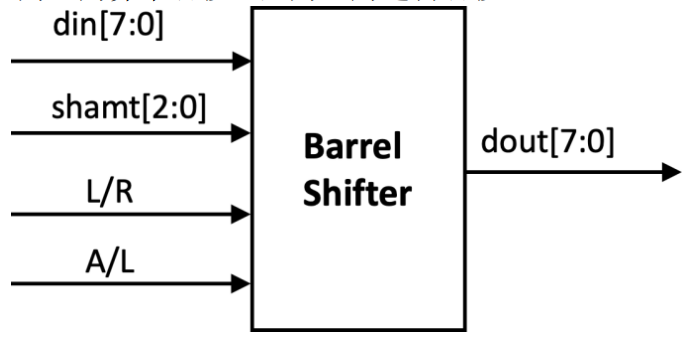
\includegraphics[width=0.8\textwidth]{6.1.png}
    \caption{桶形移位器整体方案设计}
    \end{figure}
    
    \subsubsection{顶层模块设计}
    实验电路较为简单,不需要顶层模块设计图。

    \subsubsection{引脚作用}
    \begin{table}[H]
    \centering
    \begin{tabular}{|c|c|}
        \hline
        DataIn shamt L/R A/L & 输入引脚 \\ \hline
        DataOut & 输出引脚 \\ \hline
    \end{tabular}
    \caption{桶形移位器引脚作用}
    \end{table}

    \subsubsection{原理图和电路图}
    \begin{figure}[H]
    \centering
    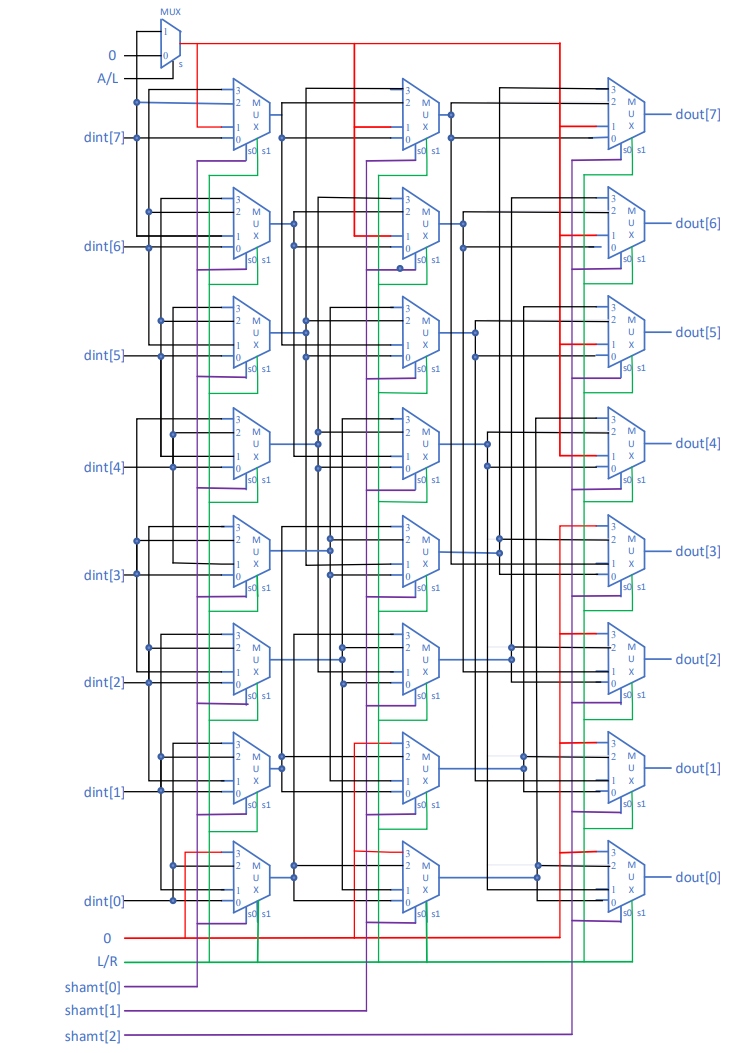
\includegraphics[width=0.8\textwidth]{6.4.1.png}
    \caption{桶形移位器原理图}
    \end{figure}

    \begin{figure}[H]
    \centering
    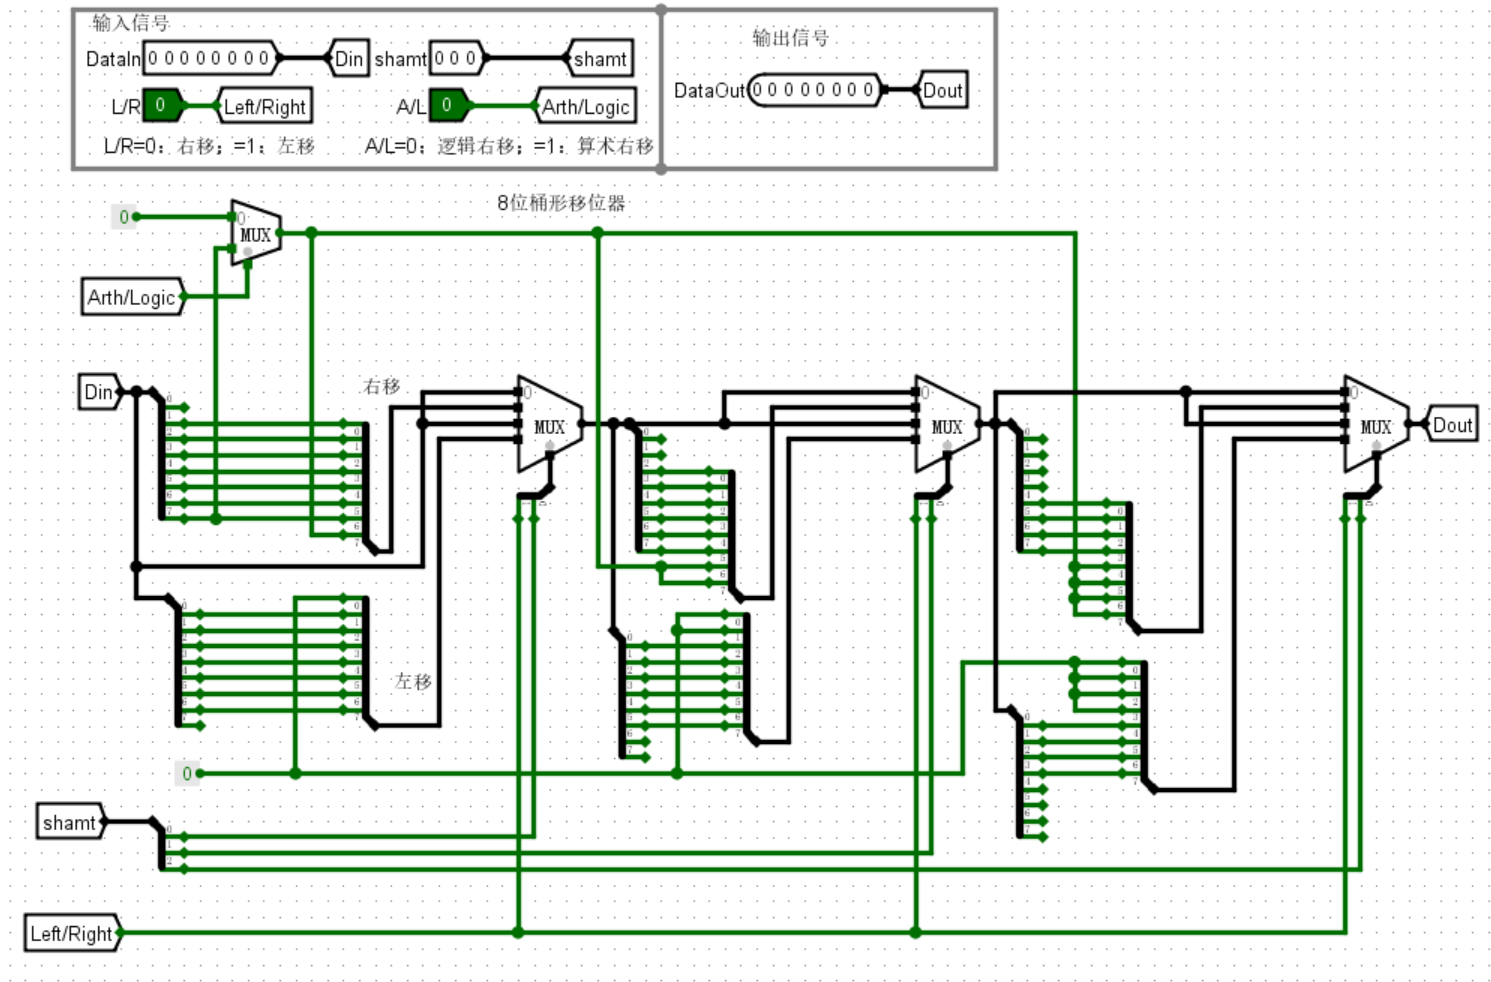
\includegraphics[width=0.8\textwidth]{6.4.2.png}
    \caption{桶形移位器电路图}
    \end{figure}

    \subsubsection{仿真测试图}
    \begin{figure}[H]
    \centering
    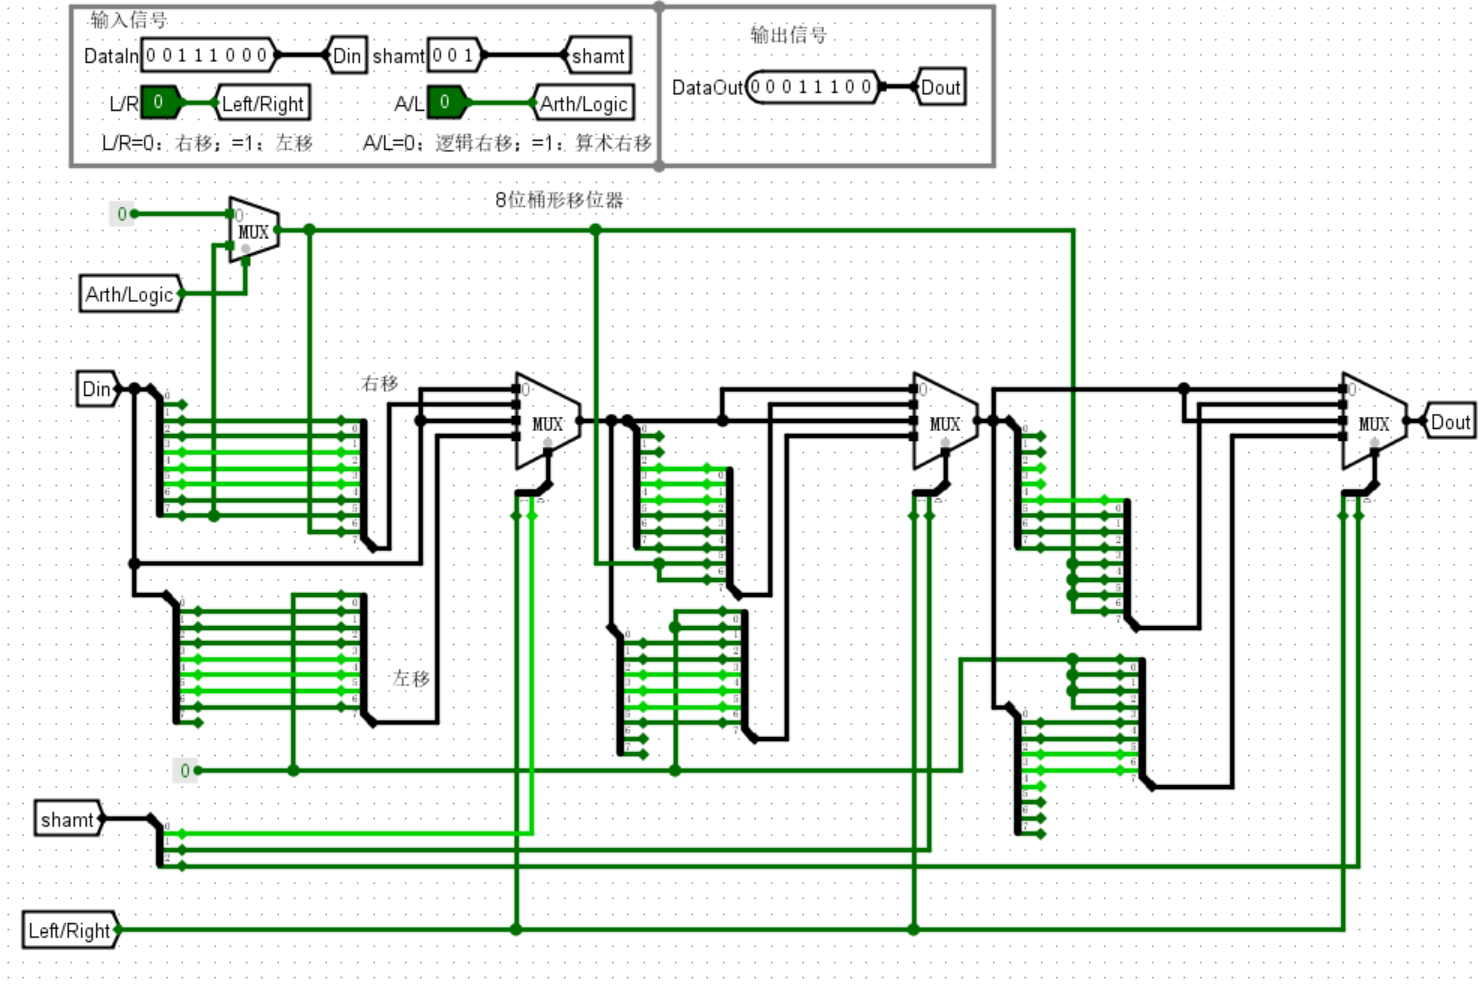
\includegraphics[width=0.8\textwidth]{6.5.1.png}
    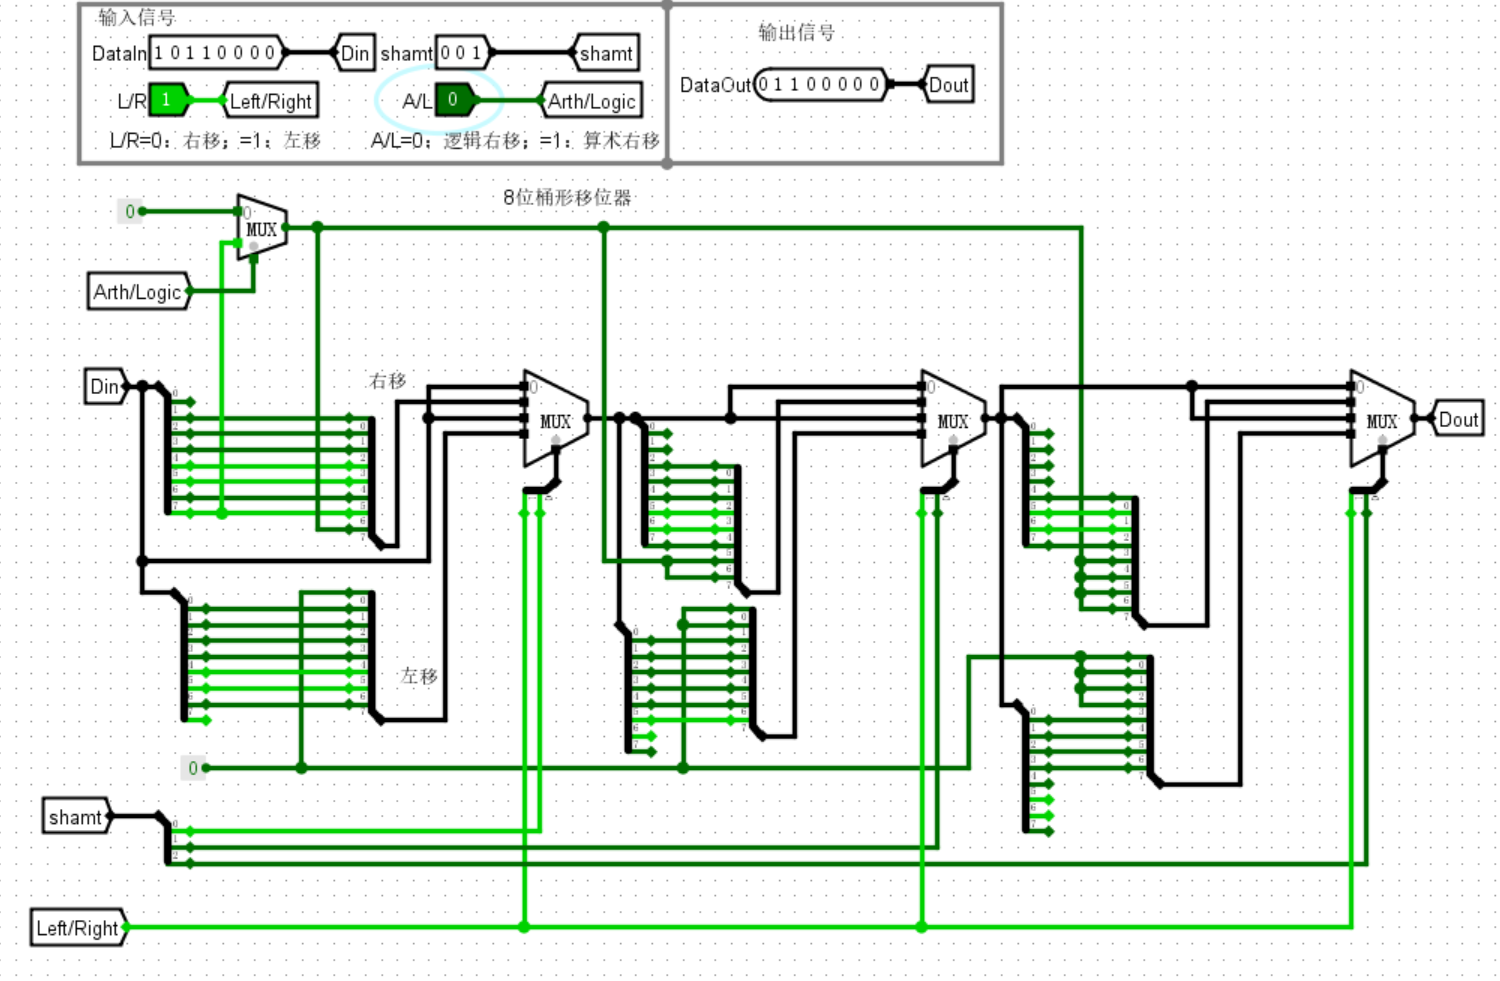
\includegraphics[width=0.8\textwidth]{6.5.2.png}
    \caption{桶形移位器仿真测试图1}
    \end{figure}

    \begin{figure}[H]
    \centering
    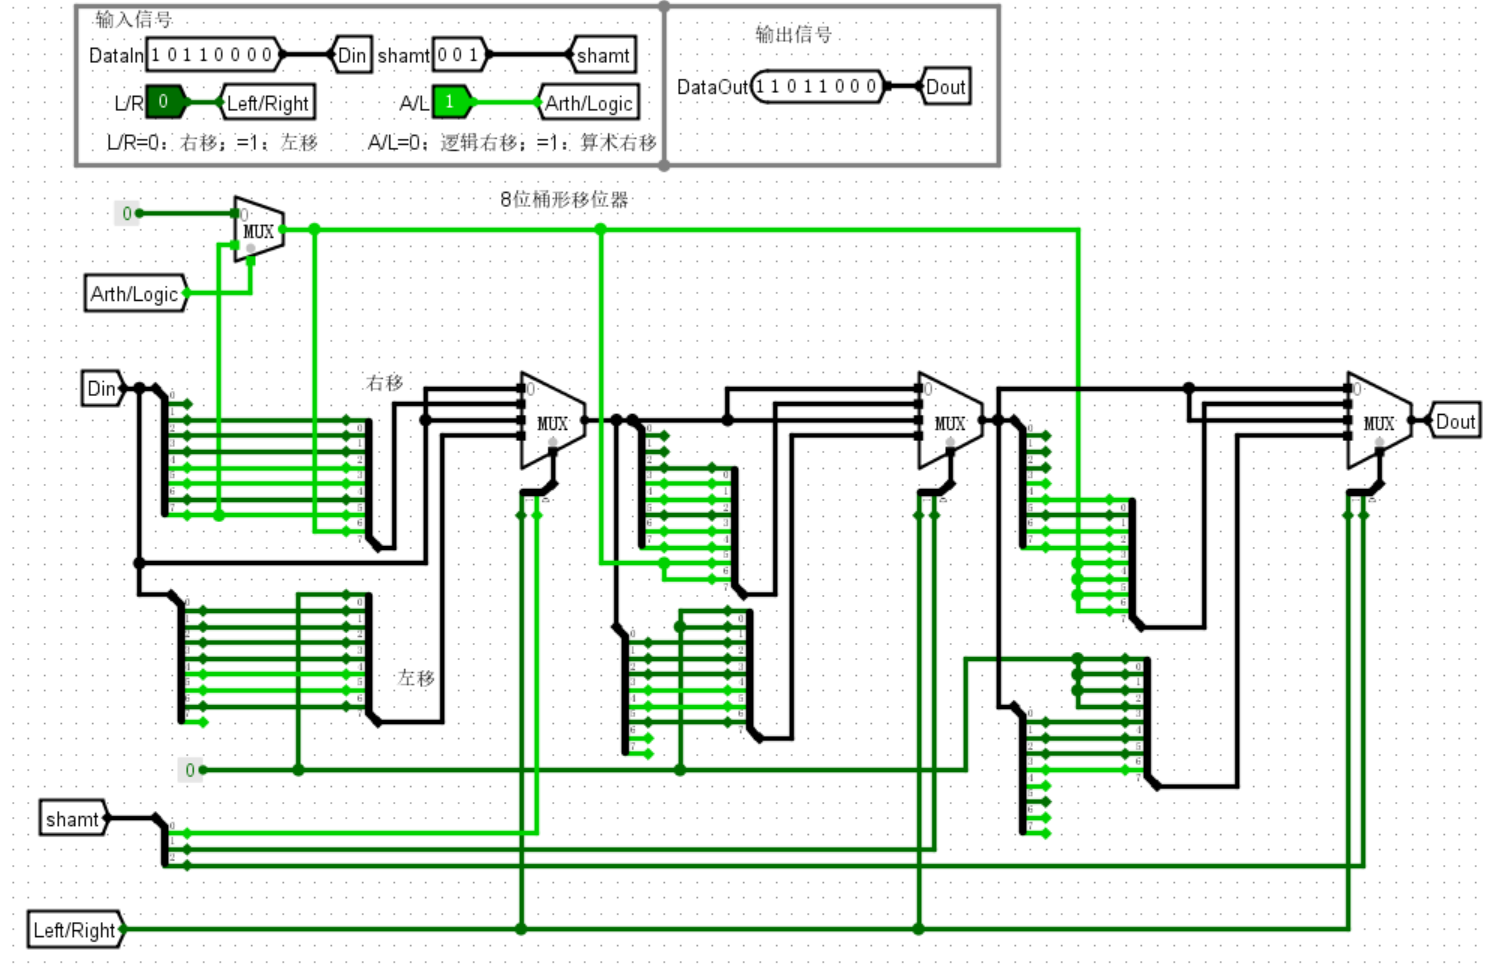
\includegraphics[width=0.8\textwidth]{6.5.3.png}
    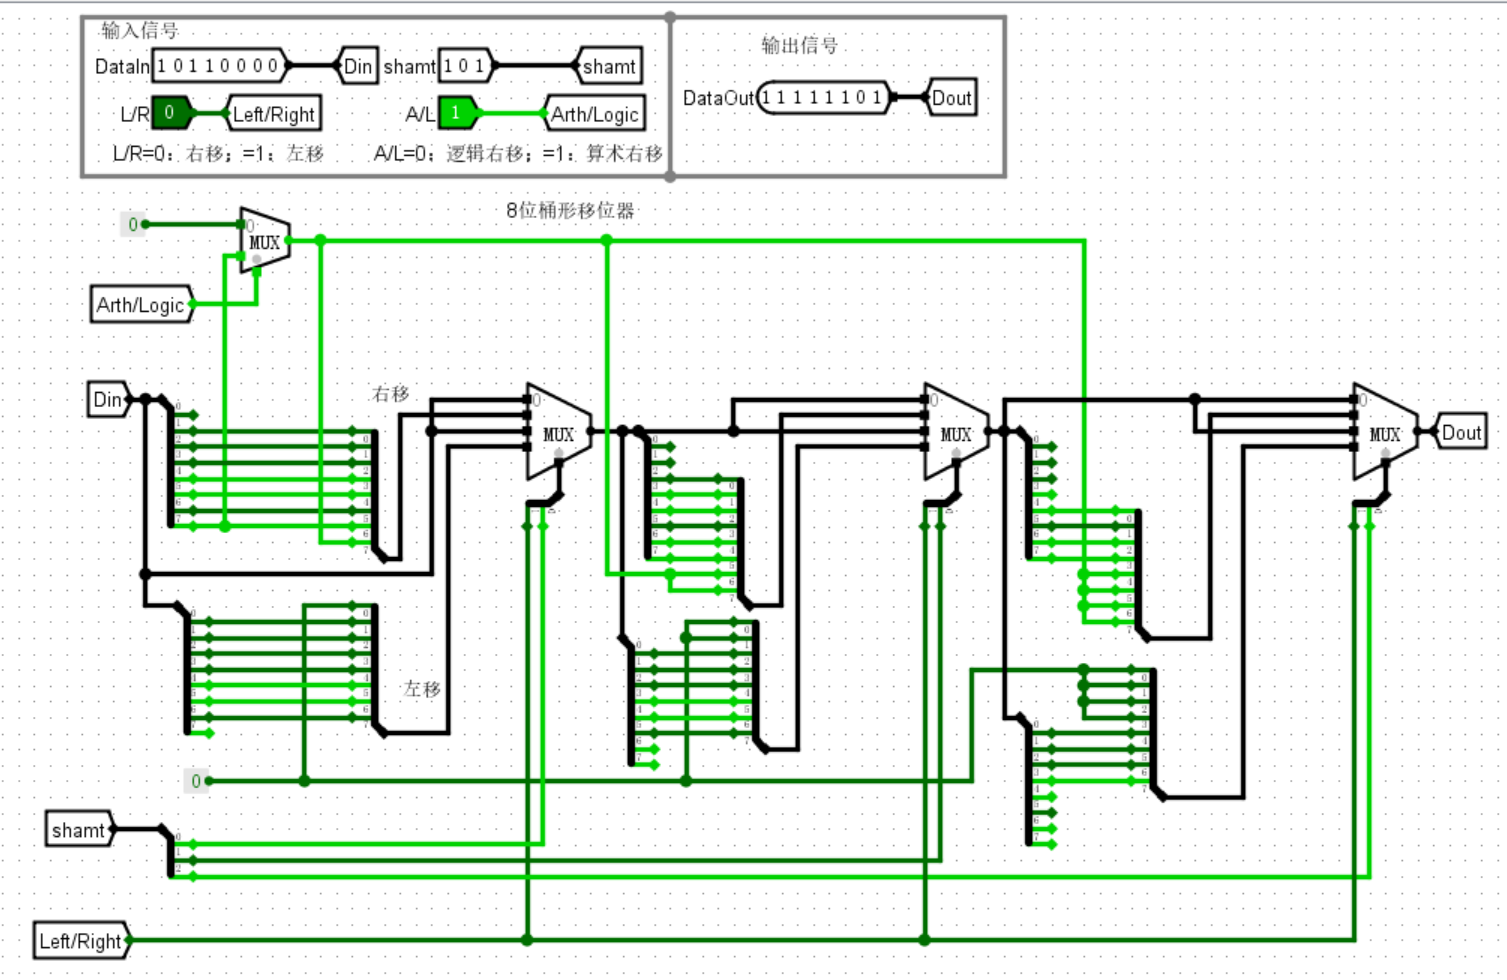
\includegraphics[width=0.8\textwidth]{6.5.4.png}
    \caption{桶形移位器仿真测试图2}
    \end{figure}
    仿真测试如下:\\
    图一DataIn为00111000,shamt为1,L/R为0,A/L为0,逻辑向右移1位,输出DataOut为00011100。\\
    图二DataIn为10110000,shamt为1,L/R为1,A/L为0,逻辑向左移1位,输出DataOut为01100000。\\
    图三DataIn为10110000,shamt为1,L/R为0,A/L为1,算术向右移1位,输出DataOut为11011000。\\
    图四DataIn为10110000,shamt为5,L/R为0,A/L为1,算术向右移5位,输出DataOut为11111101。

    \begin{table}[H]
    \centering
    \begin{tabular}{|c|c|c|c|}
        \hline
        shamt & L/R & A/L & 功能 \\ \hline
        x & 0 & 0 & 逻辑右移x位 \\ \hline
        x & 0 & 1 & 算术右移x位 \\ \hline
        x & 1 & 0 & 逻辑左移x位 \\ \hline
        x & 1 & 1 & 算术左移x位 \\ \hline
    \end{tabular}
    \caption{8位桶形移位器功能表}
    \end{table}

    \subsubsection{错误现象及分析}
    在完成实验的过程中,没有遇到任何错误。
    
    \section{思考题}

    \subsection{修改实验中的加法器电路,生成进位标志 CF、溢出标志 OF、符号标志 SF 和结果为零标志位 ZF。}
    易知$OF=C_{n}\oplus C_{n-1},SF=F_{n-1}$,$ZF =1$当且仅当$F=0$;借位/进位标志$CF=Cout\oplus Cin .$\\
    电路如图:
    \begin{figure}[H]
    \centering
    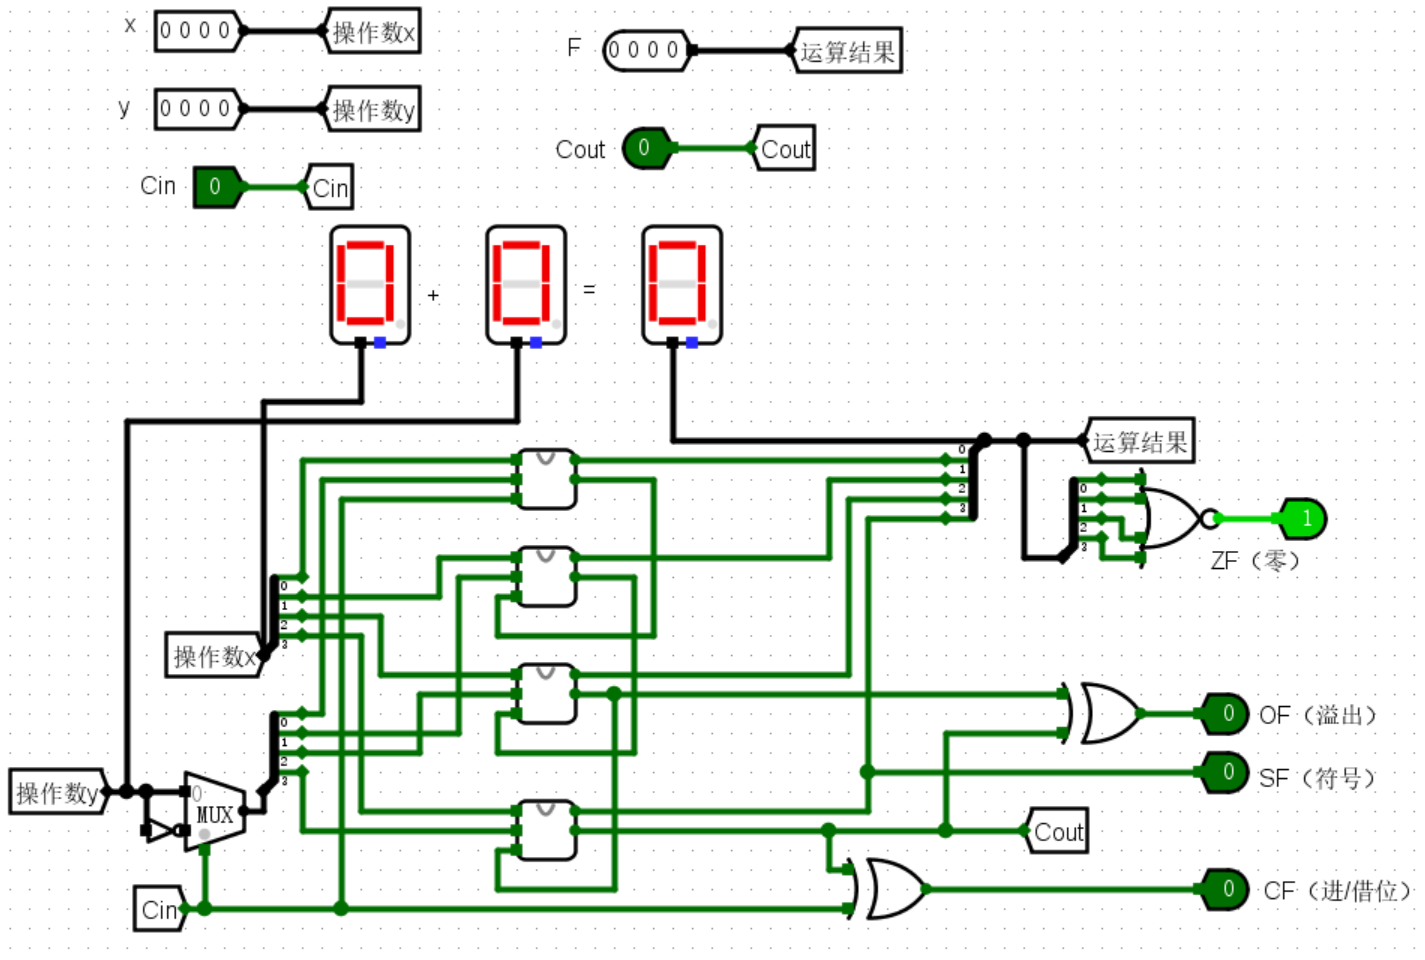
\includegraphics[width=0.8\textwidth]{7.1.png}
    \caption{带标志符加法器}
    \end{figure}
    
    \subsection{在执行比较指令时,通常使用减法运算后,判断标志位的方式来实现,试通过上述加法器实验举例说明判别的方法。}
    \begin{itemize}
        \item 对于无符号整数X和Y,计算X-Y,若CF为1,则X小于Y;若ZF为1,则X等于Y;若CF为0且ZF为0,则X大于Y。
        \item 对于带符号整数X和Y,计算X-Y,若SF为1,则X小于Y,若ZF为1,则X等于Y;若SF为0,则X大于Y。
    \end{itemize}
    
    
    \subsection{如何使用 8 位桶形移位器扩展到 32 位桶形移位器。}
    思路类似于8位桶形移位器,只是增加了shamt[3]=8,shamt[4]=16两个更多位的移位器,同时调整了分线器的输出端口,使得图形更简洁,并且对32位数据的各处位宽调整。
    采用了位扩展器减少了分线器的数量与输入端口。\\
    电路如图:
    \begin{figure}[H]
    \centering
    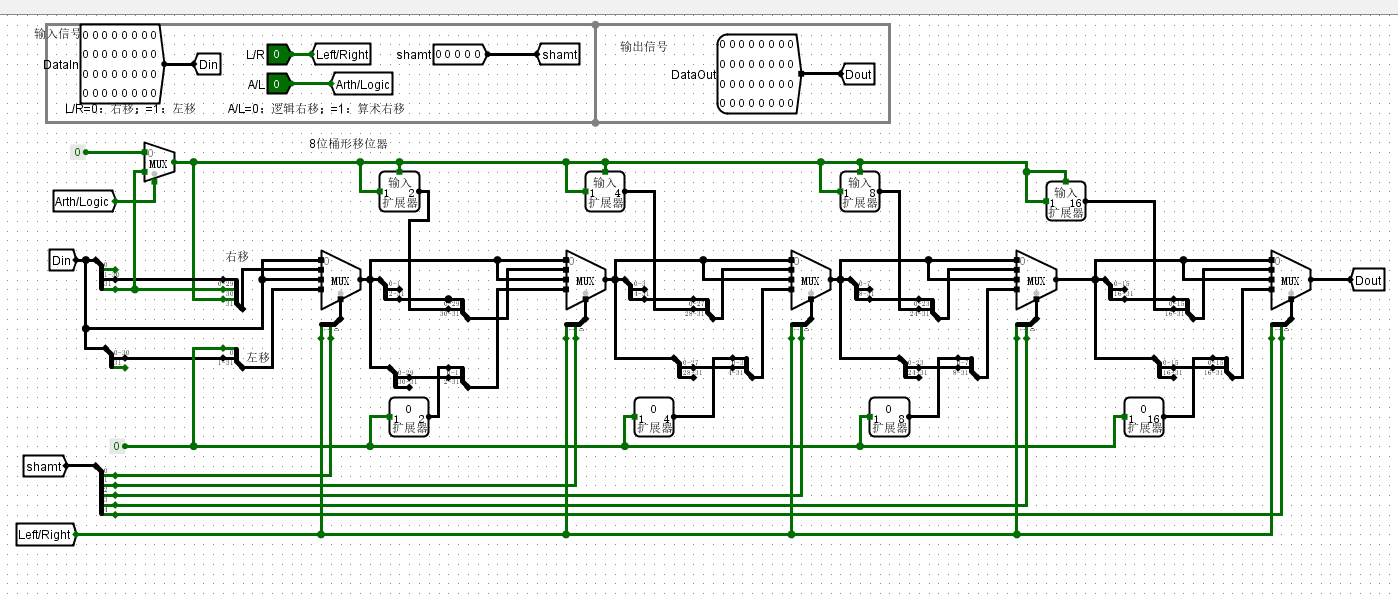
\includegraphics[width=0.8\textwidth]{9.1.png}
    \caption{32位桶形移位器}
    \end{figure}

    \subsection{Logisim 提供输出组件 LED 矩阵,通过点亮 led 灯的方式显示字符,修改 LED 矩阵行列属性为 16*16,显示“南大”两个汉字,字体可自选。}
    电路如图:
    \begin{figure}[H]
    \centering
    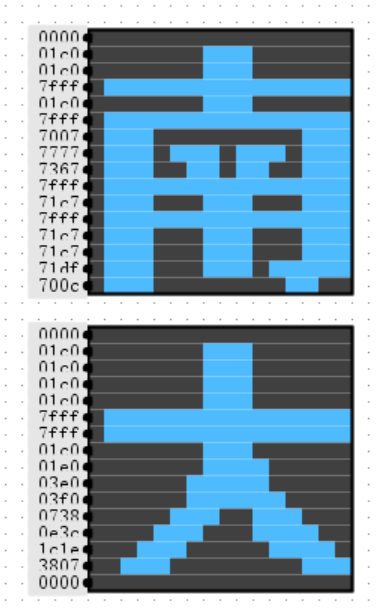
\includegraphics[width=0.8\textwidth]{10.1.png}
    \caption{"南大"LED电路}
    \end{figure}
    
\end{document}